\documentclass{apuntes}
\usepackage{changepage}

\newcounter{problem}
\newcounter{solution}
\renewcommand{\theenumi}{\alph{enumi}}

\newcommand\Problem[1][]{%
  \color{blue}
  \stepcounter{problem}%
  \ifthenelse{\isempty{#1}}{\textbf{Problema \theproblem.}}{\textbf{Problema #1.}}

  \setcounter{solution}{0}%
}

\newcommand\TheSolution{%
  \color{black}
  \textbf{Solución:}\\%
}

\newcommand\ASolution{%
  \stepcounter{solution}%
  \textbf{Solución \thesolution:}\\%
}


\setlength{\arrayrulewidth}{1mm}
\setlength{\tabcolsep}{18pt}
\renewcommand{\arraystretch}{1.5}


\newcommand{\theauthor}{}
\newcommand{\thetitle}{Sistemas Informáticos II}
\newcommand{\rightheader}{Sistemas Informáticos II}
\newcommand{\leftheader}{UAM - 2014/2015}

\title{Sistemas Informáticos II}
\author{Pedro Valero \\ Víctor de Juan \\ Eduardo Miravalls}
\date{Curso 2014 - 2015 C2}

\parindent 0in
\parskip 1em

\renewcommand{\theejr}{\arabic{chapter}.\arabic{ejr}} % IGN
\renewcommand{\theapr}{\alph{apr}} % IGN


\begin{document}

\newpage
\tableofcontents

%%%%%%%%%%%%%%%%%%%%%%%%%%%%%%%%%%%%%%%%%%%%%%%%%%%%%%%%%%%%%%%%%%%%%%%%%%

\chapter{Middleware}
Para este tema es importante tener claros varios conceptos que vamos a ir definiendo y explicando poco a poco.

\begin{defn}[Middleware]
Conjunto de aplicaciones encargadas de enlazar los componentes de un sistema distribuido.
\end{defn}

\section{Network Operating System (NOS)}
Este conjunto de aplicaciones está dividido en el protocolo específico del servicio con el que estamos trabajando (ODBC, HTTP, SMTP...), el protocolo de transporte (TCP/IP) y una capa intermedia llamada Network Operating System (NOS).

\begin{defn}[Network Operating System]
Es una extensión del sistema operativo que proporciona transparencia al cliente, para que éste realice las llamadas como si fueran locales.
\end{defn}

Algunas de las maneras de proporcionar transparencia del NOS según \concept{RM-ODP} (Open Distributed Processing Reference Model) son
\begin{itemize}
\item Ubicación: Ocultar dónde reside cada recurso (y permite que éste se mueva, incluso mientras está siendo utilizado).
\item Persistencia: Ocultar tanto la activación y desactivación de objetos como sus fallos y recuperaciones mediante la replicación.
\item Concurrencia: Ocultar la utilización de recursos concurrentes.
\item Prestaciones: Escalar el tamaño y reconfigurar el sistema para mejorar sus prestaciones según varía la carga de trabajo.
\item Espacio de nombres:
\item SSO: Single Sign On - Un único usuario y contraseña para todo el sistema.
\item Tiempo: Todos los componentes deben estar sincronizados.
\item Protocolos: Idéntica interfaz de programación para todos los protocolos de transporte.
\end{itemize}

Debido a que la representación interna de los datos es dependiente del ordenador (hardware o sistema operativo) es necesario definir un mecanismo para que, independientemente de la plataforma, la comunicación sea posible. Algunos métodos son utilizar estándares de \textbf{codificación de caracteres} (ISO-8859-1,UTF-8), \textbf{XML}, sistemas propios de aplicaciones (\textbf{RPC,XDR}) o un estándar \textbf{Abstract Synyax Notation} (con una gramática y reglas para codificar los datos).


\section{Servicios de transporte}

Una vez hablado del NOS, vamos a ver unos conceptos de  servicios de transporte del middleware.

Lo primero es recordar que hay 2 modelos de interacción, \textbf{síncrono} o \textbf{asíncrono}. Además de estos modelos, las interacciones pueden ser de tres tipos.
\begin{itemize}
	\item \textbf{R:} Petición. (El cliente hace una petición sin esperar respuesta, por ejemplo para cerrar la conexión)
	\item \textbf{RR:} Petición → Respuesta.
	\item \textbf{RRA:} Petición → Respuesta → ACK.
\end{itemize}

\subsection{API directa}

\begin{defn}[APIs directas]
API viene de \textit{Application Programming Interface} (Interfaz de programación de aplicaciones).

La utilización de APIs directas es la utilización de una interfaz de programación para acceder a unos servicios (proporcionados por la aplicación).
\end{defn}

Habitualmente son servicios de nivel de transporte o sesión. La ubicación de extremos no es transparente para el programa, ya que necesitas saber dónde está la interfaz para poder utilizarla. Para ver un ejemplo de API, consultar: \href{https://apigee.com/OneDrive/embed/console/OneDrive}{API de OneDrive}.

\subsection{Sockets}

Son la leche porque proporcionan mucha transparencia: podemos comunicarnos entre procesos sin tener ni idea de nada, simplemente es como escribir en un fichero (de hecho, si recordamos de Redes II un socket es directamente un descriptor de fichero en Linux).

Aunque ya deberíamos saberlo, incluimos un par de esquemas (sacados de las transparencias) en los que vemos cómo establecer una comunicación orientada a conexión (\ref{SocketConexion}) y una comunicación no orientada a conexión (\ref{SocketNoConexion})


\begin{figure}[hbtp]
\centering
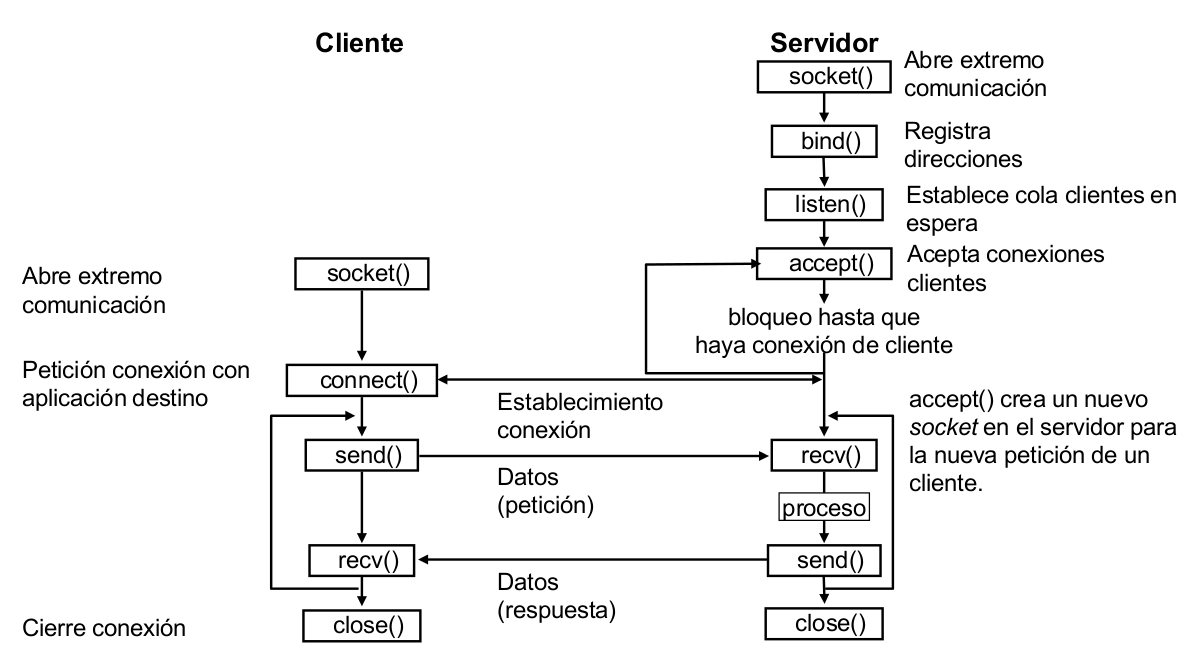
\includegraphics[width=1\textwidth]{img/SocketConexion.png}
\caption{Comunicación orientada a conexión.}
\label{SocketConexion}
\end{figure}

\begin{figure}[hbtp]
\centering
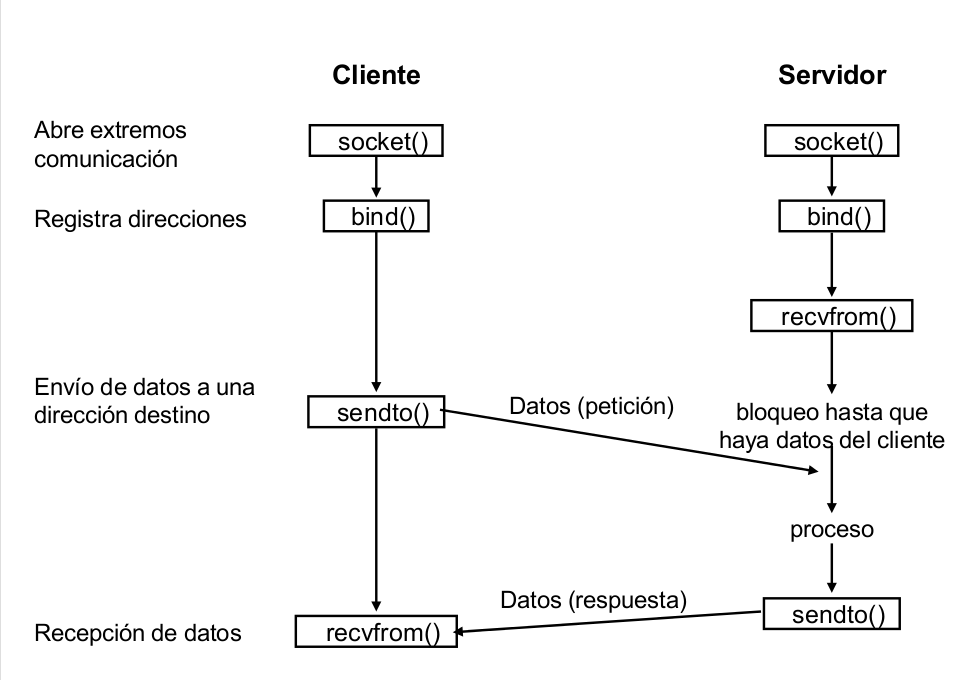
\includegraphics[width=1\textwidth]{img/SocketNoConexion.png}
\caption{Comunicación No Orientada a conexión.}
\label{SocketNoConexion}
\end{figure}
\newpage
\section{Modelos de servicios distribuidos}

La base de este curso es cómo dar servicio a muchos clientes. Si tenemos una web a la que se conectan 10 personas, nos vale con cualquier ordenador, pero ¿Cuánta gente usa google? Ni de coña google tiene un único servidor haciendo todo, tiene que tener los \textbf{servicios distribuidos}. A lo largo de esta sección iremos viendo muchas de las maneras de llevar esto a cabo.

\subsection{RPC - Remote Procedure Calls}
Este modelo se basa en realizar llamadas a funciones como si fueran locales, así el procesamiento de esa función no se realiza en local sino en remoto y nos ahorramos recursos de procesamiento.

Para el funcionamiento de RPCs necesitamos unos componentes intermedios llamados \concept{Stub}. En el siguiente diagrama se entiende perfectamente el funcionamiento de los RPCs.
\begin{figure}[htb]
\centering
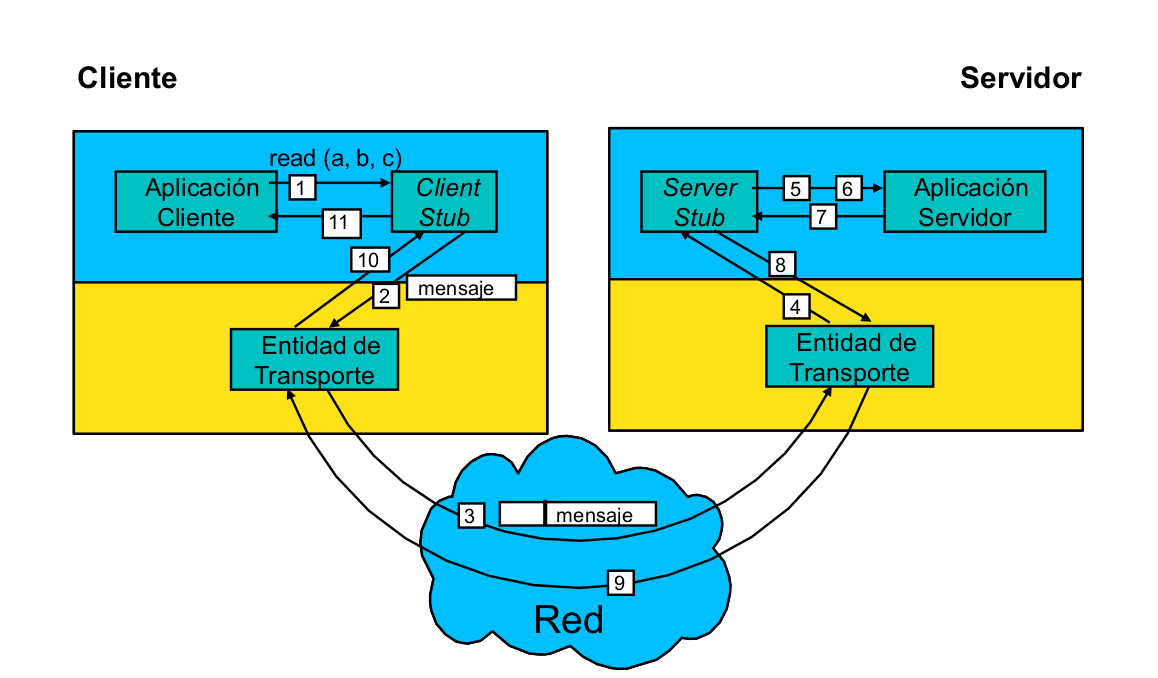
\includegraphics[width=0.9\textwidth]{img/RPC.png}
\caption{Funcionamiento de una llamada RPC.}
\label{RPCimg}
\end{figure}
\newpage

\obs La espera del cliente es \textbf{bloqueante}.

\obs Una ventaja realmente interesante de esto es la transparencia de representación de los datos. RPC (y los stubs intermedios) permiten que un cliente que utiliza Big Endian pueda pasarle los parámetros a una función que se ejecute en un servidor que utiliza Little Endian. Esta \textit{transformación} de los datos de un sistema de codificación al otro se llama \concept{Marshalling} (el codificarlos para enviar) y \concept{Unmarhsalling} (descodificarlos al recibirlos). Ambos stubs tienen que hacer marshalling y unmarshalling al enviar y recibir mensajes respectivamente.

\paragraph{Problemas de RPC}
\begin{itemize}
	\item No existe el paso de parámetros por referencia.
	\item Hay que conocer de antemano dónde está el servidor exáctamente y en qué puerto escucha.
	\subitem Para saber el puerto en el que el servidor está escuchando, éste tiene que registrarse en un \concept{PortMapper} al que el cliente pregunta por el puerto.
 	\item Tras un \textit{Time Out} No se sabe si la llamada se ha ejecutado o no. Para intentar mitigar este problema en algunos casos, encontramos estrategias distintas en las llamadas RPC:
		\subitem Ejecución Exactamente una vez.
		\subitem Ejecución Como máximo una vez.
		\subitem Ejecución Al menos una vez.\\
	Para solventar esto es necesario también saber si las operaciones son \concept{operaciones de RPC idempotentes} (se pueden ejecutar cualquier número de veces) o no\footnote{Por ejemplo un cálculo $4+4$ lo puedes ejecutar todas las veces que quieras, pero un insert en una base de datos no}.
	\item Es necesaria una representación de datos compartida por los stubs.
	\item Seguridad. ¿Y si el servidor ha sido comprometido y me va a devolver datos que me hagan mal?
\end{itemize}


\paragraph{SUN RPC: } Una de las implementaciones más comunes de RPC es \concept{Sun RPC}. Vamos a estudiarla un poco más en detalle.


Tiene 3 componentes:
\begin{itemize}
	\item \concept{XDR} Lenguaje de definición de tipos de datos. Tiene una sintaxis similar a C, pero es sólo de definición de datos, no de programación
	\item \textbf{Especificación de RPC: } Genera los \textit{stubs} y el fichero de interfaz (para ser incluido al programar)
	\item \textbf{Librería de implementación}
\end{itemize}

Sólo por si interesa, incluimos un esquema de cómo funciona y qué ficheros se generan en la codificación de un servicio utilizando RPC.


\begin{figure}[htb]
\centering
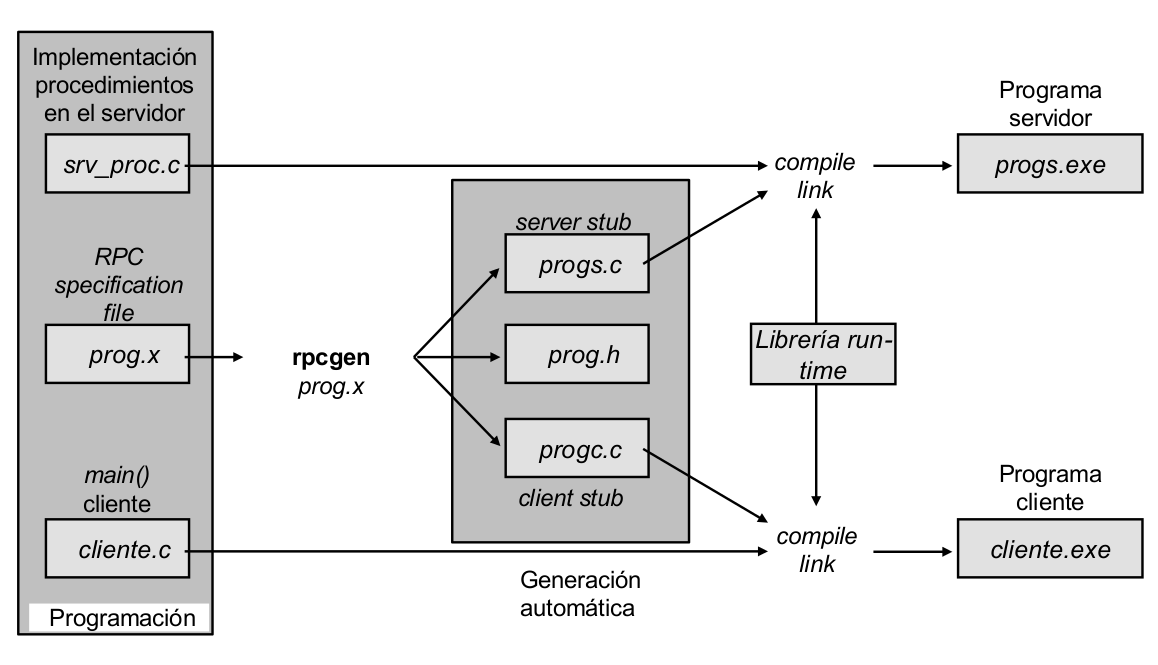
\includegraphics[width=1\textwidth]{img/SUNRPC.png}
\caption{Compilación y generación de código para Sun RPC.}
\label{SunRPC}
\end{figure}

\paragraph{Algunas diferencias entre RPCs}
\begin{itemize}
	\item Parámetros: Aunque en general soporten múltiples parámetros (\concept{Apollo RPC} por ejemplo), Sun RPC sólo tiene un único parámetro, tanto de entrada como de salida (obviamente pueden ser estructuras).
	\item Marshalling: En general lo hace el RPC, aunque en Sun RPC el marshalling que se realiza es mínimo. Es responsabilidad del usuario tener cuidado con eso.
\end{itemize}

Comentamos que Apollo RFC tiene su propio lenguaje de representación de datos, \textit{Network Data Representation} \concept{NDR} (como el XDR de Sun RPC). Apollo tiene también un lenguaje de representación de interfaces \concept{NIDL} (\textit{Network Interface Definition Language}).

\subsection{Web Services (SOAP-WSDL-UDDI)}
Es un modelo de uso de la Web. La idea es tener servidores que ofrecen servicios (localizar geográficamente a través de la IP, ofrecer información de finanzas...) y que cualquiera puede requerir esos servicios. ¿Qué diferencia tiene con RPC? Que en RPC el programador tiene que codificar el lado del servidor y tener conciencia de como funciona, mientras que con los WebServices, el programador que está haciendo un cliente puede utilizar los servicios que le proporciona un servidor que otro programador haya hecho en cualquier otro momento.

Añade un nivel más de transparencia, ya que el programador del cliente no tiene ni idea de cómo funciona el WebService.

La \textbf{función del middleware} aquí es proporcionar funcionalidad para publicar los servicios que ofreces y descubrir los nuevos servicios que vayan surgiendo. Además, tiene que permitir que los servidores soliciten servicios también (multi-\textit{tier}).

\paragraph{Complementos de los Web Services} \concept{OASIS} (Organization for the Advancement of Structured Information Standards) está trabajando (y ha trabajado) en estandarizar una serie de complementos útiles para la mejor utilización de los Web Services y una serie de familia de especificaciones:
\begin{itemize}
\item Complementos:
	\subitem Seguridad.
	\subitem Fiabilidad.
	\subitem Addresing: describir las direcciones de emisor y receptor de un mensaje dentro del propio mensaje.
	\subitem Transaction.
\item \concept{WSRL} - Web Services Resource Framework.
	\subitem WS-Resource (Conjunto de un recurso y un Web Service a través del cual se accede a él.
	\subitem WS-ResourceProperties
	\subitem WS-ResourceLifetime
	\subitem WS-BaseFaults (mecanismo extensible para gestionar errores)
	\subitem WS-ServiceGroup
\end{itemize}

Los WebServices necesitan de 3 protocolos estándares. En el siguiente gráfico se muestran los componentes y protocolos de comunicación utilizados en los WebServices.


\begin{figure}[htb]
\centering
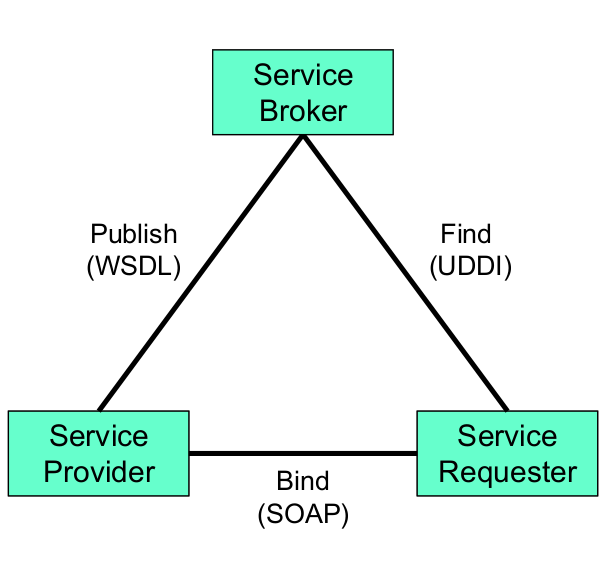
\includegraphics[width=0.9\textwidth]{img/WS.png}
\caption{Componentes de un WS para su funcionamiento.}
\label{WSimg}
\end{figure}


\subsubsection{SOAP}
\begin{defn}[SOAP]
(siglas de Simple Object Access Protocol) Es un protocolo estándar que define cómo dos objetos en diferentes procesos pueden comunicarse por medio de intercambio de datos XML.

Es independiente de la plataforma y el lenguaje de programación y, aunque se puede usar en distintos sistemas de mensajes y sobre distintos protocolos de transporte, su uso principal es transportar RPCs sobre HTTP.
\end{defn}

Un mensaje SOAP es un documento XML ordinario con una estructura definida en la especificación del protocolo. Dicha estructura la conforman las siguientes partes:
\begin{itemize}
\item \textbf{Envelope (obligatoria)}: Raíz que da la estructura, es la parte que identifica al mensaje SOAP como tal.
\item \textbf{Header}: Esta parte es un mecanismo de extensión ya que permite enviar información relativa a cómo debe ser procesado el mensaje. Es una herramienta para que los mensajes puedan ser enviados de la forma más conveniente para las aplicaciones. El elemento "Header" se compone a su vez de "Header Blocks" que delimitan las unidades de información necesarias para el header.
\item \textbf{Body (obligatoria)}: Contiene la información relativa a la llamada y la respuesta.
\item \textbf{Fault}: Bloque que contiene información relativa a errores que se hayan producido durante el procesado del mensaje y el envio desde el "SOAP Sender" hasta el "Ultimate SOAP Receiver"
\end{itemize}

\subsubsection{WSDL}
\begin{defn}[WSDL]
WSDL son las siglas de Web Services Description Language, un formato XML que se utiliza para describir servicios Web.

WSDL describe la interfaz pública de los servicios Web. Está basado en XML y describe la forma de comunicación, es decir, los requisitos del protocolo y los formatos de los mensajes necesarios para interactuar con los servicios listados en su catálogo. Las operaciones y mensajes que soporta se describen en abstracto y se ligan después al protocolo concreto de red y al formato del mensaje
\end{defn}

Estructura de una declaración WSDL
\begin{itemize}
\item \textbf{definitions}: Elemento raíz que contiene el resto. Define su
nombre y los espacios de nombres que utiliza.
\item \textbf{types}: Tipos de datos utilizados entre cliente y servidor. Usa
W3C XML Schema (XSD) por defecto.
\item \textbf{message}: Declaraciones de mensajes empleados para
peticiones y respuestas y los elementos que los forman.
\item \textbf{portType}: Operaciones soportadas y encadenamiento de
mensajes que implica su ejecución.
\item \textbf{binding}: Modo en que los mensajes se transmiten sobre un
protocolo de RPC, con extensiones específicas para SOAP.
\item \textbf{service}: Contiene la información de la dirección en la que se
localiza el servicio.

\end{itemize}

\subsubsection{UDDI}
\begin{defn}[UDDI]
UDDI son las siglas del catálogo de negocios de Internet denominado Universal Description, Discovery and Integration. El registro en el catálogo se hace en XML. UDDI es una iniciativa industrial abierta (sufragada por la OASIS) entroncada en el contexto de los servicios Web.
\end{defn}

Consta de 3 partes: \textbf{modelo de datos} (esquema XML), la \textbf{API} (RPCs con SOAP para registrar y buscar servicios) y los \textbf{Cloud Services} (los servidores que proporcionan el servicio).

El registro de un negocio en UDDI distingue tres categorías de datos:
\begin{itemize}
\item \textbf{Páginas blancas}. Dirección, contacto y otros identificadores conocidos.
\item \textbf{Páginas amarillas}. Categorización industrial basada en taxonomías.
\item \textbf{Páginas verdes}. Información técnica sobre los servicios que aportan las propias empresas.
\end{itemize}
UDDI es uno de los estándares básicos de los servicios Web cuyo objetivo es ser accedido por los mensajes SOAP y dar paso a documentos WSDL, en los que se describen los requisitos del protocolo y los formatos del mensaje solicitado para interactuar con los servicios Web del catálogo de registros.


\paragraph{Ventajas e inconvenientes de los Web Services}

\textbf{Ventajas}
\begin{itemize}
\item Aportan interoperabilidad entre aplicaciones de software independientemente de sus propiedades o de las plataformas sobre las que se instalen.
\item Los servicios Web fomentan los estándares y protocolos basados en texto, que hacen más fácil acceder a su contenido y entender su funcionamiento.
\item Permiten que servicios y software de diferentes compañías ubicadas en diferentes lugares geográficos puedan ser combinados fácilmente para proveer servicios integrados.
\end{itemize}


\textbf{Inconvenientes}
\begin{itemize}
\item Para realizar transacciones no pueden compararse en su grado de desarrollo con los estándares abiertos de computación distribuida como CORBA (Common Object Request Broker Architecture).
\item Su rendimiento es bajo si se compara con otros modelos de computación distribuida, tales como RMI (Remote Method Invocation), CORBA o DCOM (Distributed Component Object Model). Es uno de los inconvenientes derivados de adoptar un formato basado en texto. Y es que entre los objetivos de XML no se encuentra la concisión ni la eficacia de procesamiento.
\item Al apoyarse en HTTP, pueden esquivar medidas de seguridad basadas en firewall cuyas reglas tratan de bloquear o auditar la comunicación entre programas a ambos lados de la barrera.
\end{itemize}

\subsection{REST}
\begin{defn}[REST]
Si bien el término REST se refería originalmente a un conjunto de principios de arquitectura, en la actualidad se usa en el sentido más amplio para describir cualquier interfaz web simple que utiliza XML y HTTP, sin las abstracciones adicionales de los protocolos basados en patrones de intercambio de mensajes como el protocolo de servicios web SOAP.

Es posible diseñar sistemas de servicios web de acuerdo con el estilo arquitectural REST de Fielding y también es posible diseñar interfaces XMLHTTP de acuerdo con el estilo de llamada a procedimiento remoto (RPC), pero sin usar SOAP.

Estos dos usos diferentes del término REST causan cierta confusión en las discusiones técnicas, aunque RPC no es un ejemplo de REST.
\end{defn}

Al trabajar con REST se considera que el sistema se compone de \textbf{recursos}, es decir, elementos que deben ser accedidos en el sistema distribuído y a los que se accede a través de su identificador global \concept{URI}.

La idea es utilizar los métodos de HTTP para acceder a los recursos y servicios del servidor. El servidor define su interfaz normalmente utilizando \concept{WADL} \textit{Web Application Description Language}. El programador del cliente tiene que saberse la especificación concreta, y saber qué objetos recibe qué peticiones.

Para entender mejor REST, miramos el ejemplo de la API de onedrive:

\begin{figure}[hbtp]
\centering
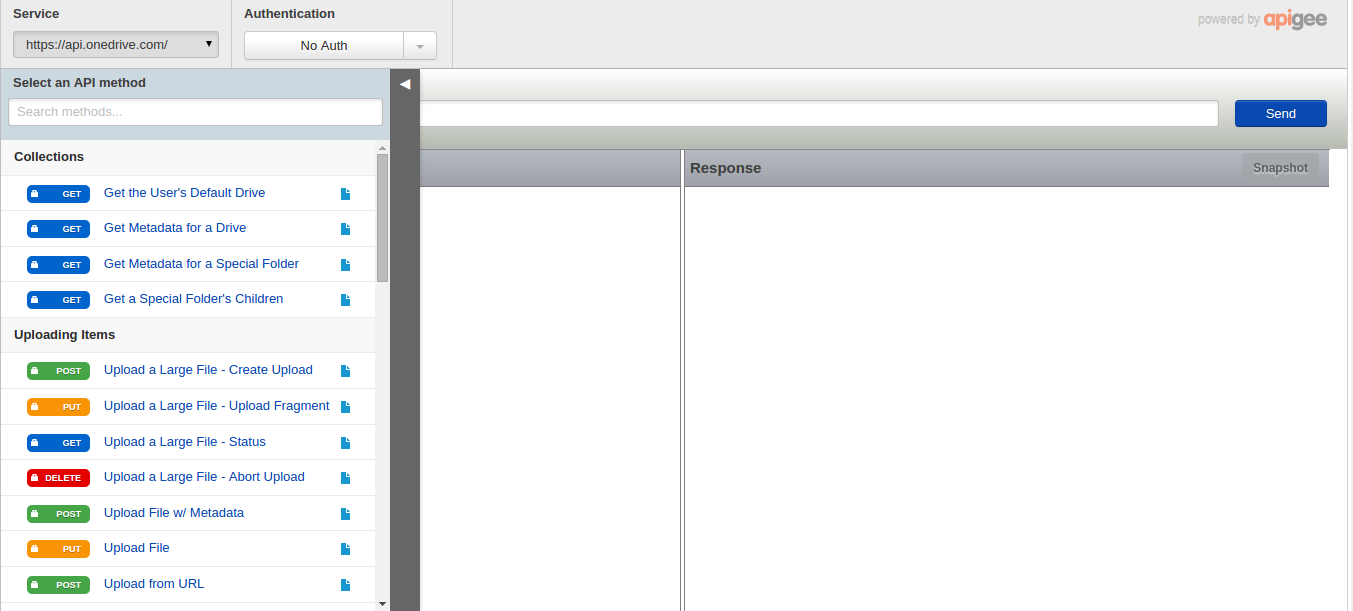
\includegraphics[width=1\textwidth]{img/REST.png}
\caption{API de OneDrive utilizando REST.}
\label{REST}
\end{figure}

Aquí están descritas las posibilidades que existen en el servidor de OneDrive. Con simples peticiones HTTP podemos funcionar. La petición \textit{https://api.onedrive.com/v1.0/drive/} (un GET de HTTP normal) nos devolvería el directorio con las carpetas que tiene el usuario con el que nos hayamos autenticado antes. ¿Cómo autenticarse? Con una petición POST con los datos pertinentes. ¿Y cómo nos devuelve los datos? Lo más habitual es en formato \textbf{JSON} aunque también puede ser en XML.

La utilización de HTTP y JSON/XML hace posible la programación de clientes en cualquier plataforma y es una comunicación más ligera que SOAP. Un inconveniente es que es menos ``transparente''\footnote{transparente en el sentido de que no te enteras de nada. Para utilizar REST tienes que saber más del servicio que utilizas.}.

\textbf{REST es una arquitectura, no un estándar.}


\subsection{Comuncación mediante colas de mensajes}

\begin{defn}[MOM]
Message Oriented Middleware.

Es un proceso asíncrono en el que se genera un mensaje, se encola y se sigue lo que se estaba. Como mandar un correo electrónico, que se encola en la bandeja de entrada y tu sigues trabajando.
\end{defn}

Las conexiones en colas de mensajes pueden ser 1-1, 1-N, N-1 y N-M.

\paragraph{Situaciones ideales}
\begin{itemize}
 	\item Conexiones no permanentes y costosas.
 	\item Múltiples servidores procesando mensajes de clientes.
 	\item Llegada de mensajes impredecibles o en ráfagas
 	\item Sistemas de tipo publicación/suscripción.
 \end{itemize}
 \obs Permite balanceo automático de carga en un sistema distribuido. Se pueden procesar los mensajes con prioridades, no necesariamente FIFO.

Vamos a ver algunos ejemplos de gestores de colas.
\subsubsection{IBM Web Sphere MQ}
Es el MOM más extendido. Es multiplataforma y multiprotocolo.


\concept{IBM Sphere MQ} está formado por
\begin{itemize}
	\item Gestores de colas, encargados de manejar el envío y recepción de los mensajes, además de crear y gestionar el resto de los elementos.

	Tiene una API con
	\subitem Message Queuing Interface (MQI)
	\subitem Application Messagin Interface (AMI)
	\subitem Java Messaging Services (JMS)
	\item Colas de mensajes de múltiples tipos.
	\item Canales de comunicación: Conexiones unidireccionales entre gestores de colas.
\end{itemize}

A continuación mostramos un esquema de funcionamiento de un sistema de mensajería de colas:


\begin{figure}[hbtp]
\centering
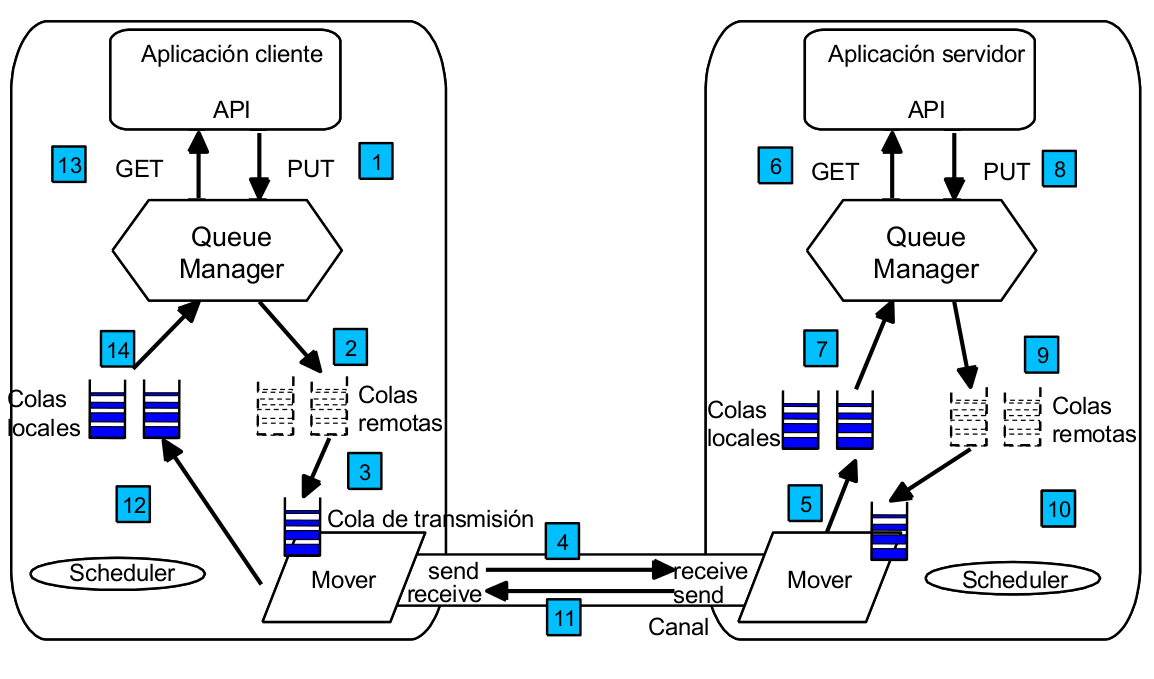
\includegraphics[width=1\textwidth]{img/MOMGen.png}
\caption{Sistema de mensajería de colas.}
\label{MOMGen}
\end{figure}
\newpage

Vemos que se distinguen 3 tipos de colas, las locales (del propio sistema) y las remotas, que el sistema reconoce que pertenecen a otro sistema y entonces el mensaje tiene que ser enviado al sistema al que pertenece la cola remota.

Además de estos 3 tipos de colas (locales, remotas y de transmisión) podemos definir en nuestras colas un par de propiedades: persistentes o temporales (en el almacenamiento de los mensajes) y estáticas (definidas permanentemente) o dinámicas (creadas por aplicaciones). Las colas dinámicas se crean a partir de una cola modelo.

También existen las colas de activación, y de cartas muertas (con mensajes que no se han podido entregar)


En resumen, los tipos de colas pueden ser:
\begin{itemize}
	\item Local - remota.
	\item Persistente - temporal.
	\item Estática - dinámica.
	\item Activación.
	\item Cartas muertas.
	\item Transmisión.
\end{itemize}

\begin{example}
Una de las utilidades de MOM son los servicios de publicación/suscripción. A continuación incluimos un esquema que muestra perfectamente cómo funcionan este tipo de sistemas.


\begin{figure}[hbtp]
\centering
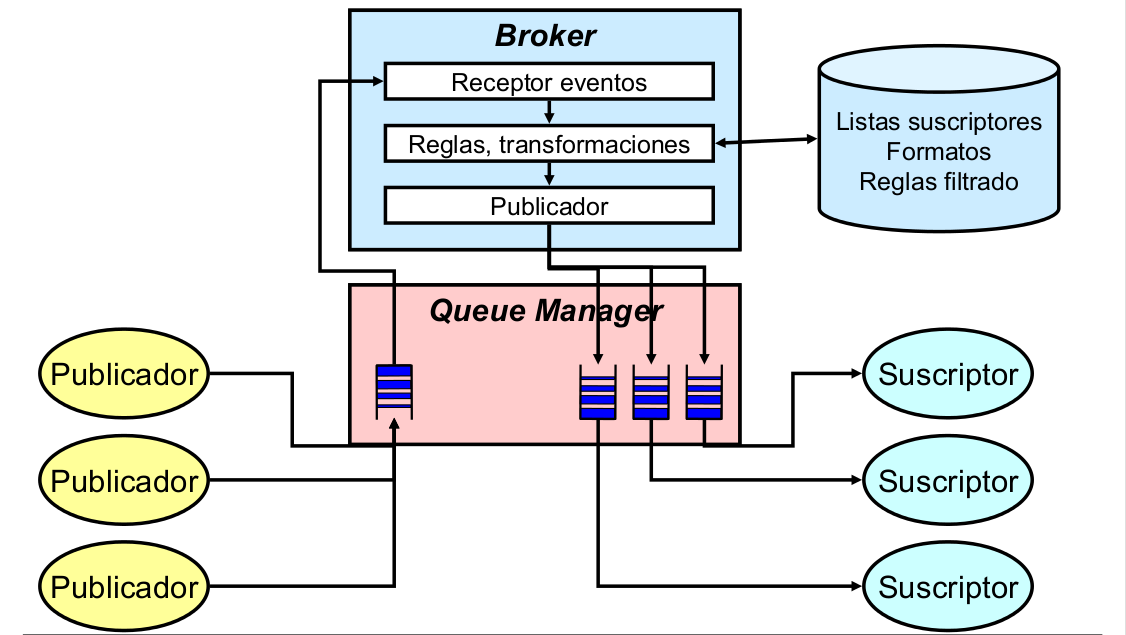
\includegraphics[width=1\textwidth]{img/PubSusc.png}
\caption{Sistema publicador/suscriptor.}
\label{PubSusc}
\end{figure}
\newpage
\end{example}


\section{Services Oriented Architecture SOA}
\subsection{ESB - Enterprise Services Bus}

Extendiendo el modelo de publicador/suscriptor tenemos un ESB. El ESB actúa como proceso centralizador de solicitudes de los clientes (normalmente mensajes o solicitudes de ejecución de acciones tipo RPC – Web Services) para su distribución a los servidores.


\begin{figure}[hbtp]
\centering
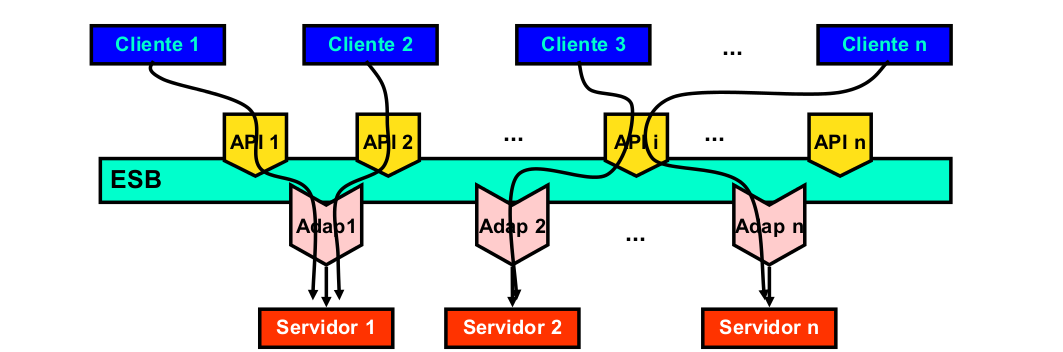
\includegraphics[width=1\textwidth]{img/ESB.png}
\caption{Enterprise Service Bus.}
\label{ESB}
\end{figure}

A continuación, estudiamos las ventajas e inconvenientes que puede tener un sistema como este:
\paragraph{Ventajas:}
\begin{itemize}
\item Adaptación rápida en entornos existentes.
\item Flexibilidad. Fácil de adaptar a nuevos requerimientos.
\item Basado en estándares.
\item Existencia de tipos de servicios y APIs predefinidas y listas para su uso.
\item Convierte tareas de programación en configuración (manipulación de datos, por ejemplo).
\item Facilita la gestionabilidad del sistema, al proporcionar un punto único de control para todos los intercambios.
\end{itemize}
\paragraph{ Inconvenientes:}
\begin{itemize}
\item Posible punto único de fallo.
\item Fácil saturación del ESB a cargas altas de comunicación.
\item Sin una planificación correcta de APIs y conectores no evita la conexión lógica punto a punto entre clientes y servidores, sólo la física.
\item Requiere más sistemas en ejecución, para soportar el propio ESB.
\item Introducción de un elemento adicional en la cadena de procesamiento, con lo cual el rendimiento se puede ver afectado.
\item Escasas ventajas para entornos sencillos. Estas se ven más en situaciones complejas, con muchos tipos de clientes y servidores.
\end{itemize}

\subsection{RMI - Remote Method Invocation}

Igual que en programación estructurada podíamos ejecutar funciones remotamente (con RPC), con la programación orientada a objetos (POO) también podemos tener localmente una referencia a un objeto remoto y ejecutar métodos del objeto remoto. Para ello es necesario disponer de un middleware espefícico, con unos módulos de comunicación y de referencia remota.


\begin{figure}[hbtp]
\centering
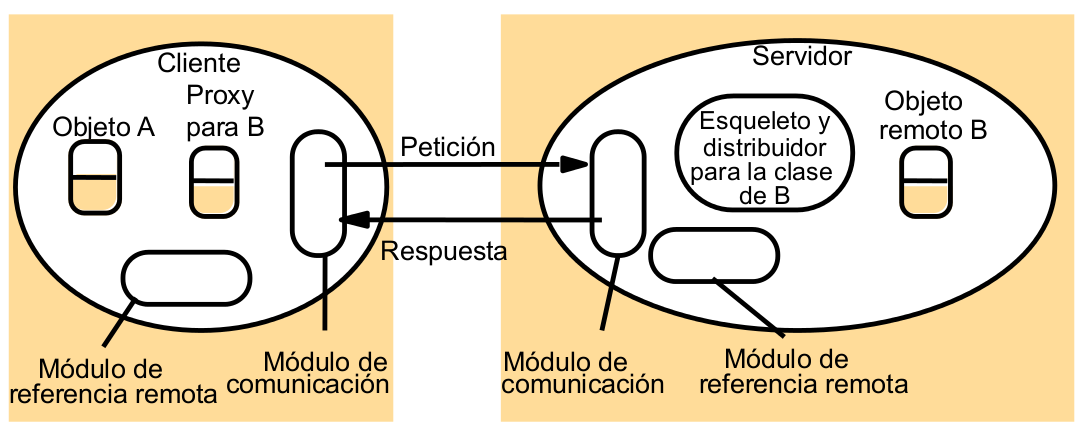
\includegraphics[width=1\textwidth]{img/RMI.png}
\caption{Esquema de funcionamiento de RMI.}
\label{RMI}
\end{figure}

En RMI también es necesario realizar marshalling y unmarshalling. El componente encargado de hacerlo es el esqueleto (del objeto remoto).

El otro componente que merece mención es el módulo de la referencia remota. El objeto que tiene el cliente es una referencia que el módulo de referencias remotas se encarga de traducir la referencia local (a algo remoto) a una referencia remota (al objeto remoto).

Aparte del RMI de Java, existen otras alternativas, como \concept{CORBA} (Common Object Request Broker Architecture) creada por \concept{OMG} (Object Management Group) y \concept{DCOM} (Distributed Component Object Model) creada por Microsoft.

\subsubsection{OMA}
\begin{defn}[OMA]
Object Management Architecture.

Establece 2 modelos. Un modelo de objetos y uno de referencias.
\end{defn}

Vamos a ver el modelo de referencias.


\begin{figure}[hbtp]
\centering
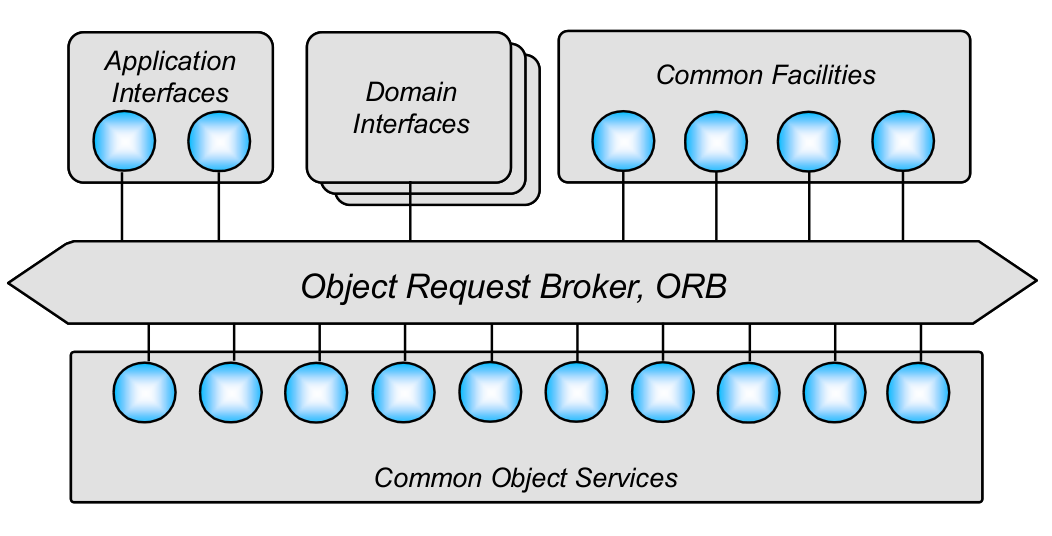
\includegraphics[width=1\textwidth]{img/OMA_Ref.png}
\caption{Esquema de funcionamiento del modelo de referencias de OMA.}
\label{OMAimg}
\end{figure}

\begin{itemize}
	\item \textit{Object Request Broker, ORB:} Bus de comunicación entre objetos.
	\item \textit{Common Object Services:} Gestión del ciclo de vida, persistencia, resolución de nombres, tiempo, control de concurrencia, seguridad...
	\item \textit{Common Facilities:} Colecciones de componentes, con funciones de tipo general, pero orientados a aplicaciones finales en vez de al sistema.
	\item \textit{Domain Interfaces:} Colección de componentes/objetos comunes específicos para áreas de aplicaciones: comercio electrónico, telecomunicaciones, banca, salud, fabricación...
	\item \textit{Application Interfaces:} Interfaces específicas de aplicaciones concretas.
\end{itemize}

\begin{defn}[ORB]
Object Request Broker → Bus de comunicación entre objetos.

Es un middleware avanzado que es la repera y permite :

\begin{itemize}
	\item Permite llamadas estáticas y dinámicas a objetos. Incluye descubrimiento dinámico de objetos.
	\item Describir las interfaces independientemente del lenguaje de programación. El lenguaje de descripción se llama \concept{IDL}\label{IDL} (Interface Description Language)
	\item Enlace directo de aplicaciones escritas en múltiples lenguajes de alto nivel (no necesariamente orientados a objetos).
	\item Sistema auto-descrito. Genera meta-información consultable dinámicamente.
	\item Soporte de seguridad,transacciones y autenticación de las comunicaciones
	\item Polimorfismo en la ejecución de funciones asociadas a un mismo mensaje.
\end{itemize}
\end{defn}

\begin{defn}[IDL]
Interface description language.
\end{defn}

Del código IDL se crean los stubs necesarios (cliente y servidor\footnote{Los stubs de servidor se llaman \textit{skeletons}}) y los ficheros de definiciones. Además, se genera código fuente del lenguaje elegido, definido en CORBA.

Este es el esquema de desarrollo de un sistema con CORBA.


\begin{figure}[hbtp]
\centering
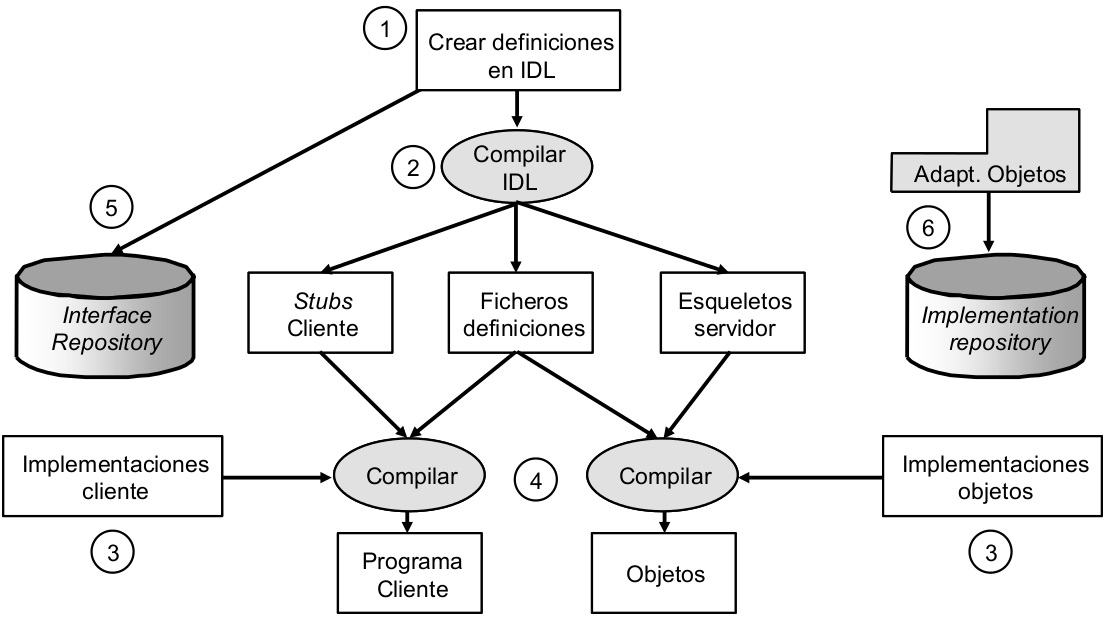
\includegraphics[width=1\textwidth]{img/CORBA.png}
\caption{Esquema del desarrollo de CORBA.}
\label{OMA}
\end{figure}


\subsubsection{Microsoft COM}

\begin{defn}[Microsoft COM]
	Microsoft Component Object Model - Plataforma de objetos de microsoft.
\end{defn}

Esta plataforma de objetos ha ido mejorandose y evolucionando a lo largo del tiempo. Primero fue \concept{DDE} (Dynamic Data Exchange) que mejoró la comunicación entre aplicaciones con \concept{OLE} (Object Linking and Embedding) hasta llegar a \textbf{COM}, con su versión de objetos distribuida \concept{DCOM} y por último, al integrarlo con MTS y MSMQ se ha llegado a \textbf{COM+}

\begin{defn}[MTS]
	Microsoft Transaction Server
\end{defn}

\begin{defn}[MSMQ]
	Microsoft Message Queueing
\end{defn}

\paragraph{Características}
Un objeto COM es un objeto en el mismo sentido que en CORBA,  es independiente del lenguaje de programación y cada objeto tiene una o varias interfaces. Estas interfaces se definen con el Lenguaje de Definición de Interfaces de Microsoft (en inglés \concept{MIDL}). Este lenguaje está basado en el IDL\ref{IDL} del \textit{Distributed Computing Environment} (\concept{DCE}) que utiliza Apollo RFC.

Los sistemas COM se organizan en componentes COM que son módulos binarios (ejecutables o librerías dinámicas). Estos módulos pueden contener uno o varios objetos COM, una interfaz gráfica e incluso otro componente\footnote{Si un componente incluye a otro, el grande se llama componente \textit{ActiveX}}

\paragraph{Funcionalidades}

\begin{itemize}
	\item Transparencia de la localización de los objetos.
	\item Activación de los objetos a distancia (a través del \concept{SCM} (\textit{Service Control Manager})
	\item Seguridad en las comunicaciones (\concept{NTLMP} (\textit{NT Lan Manager Protocol}) y \concept{SAM} (\textit{Security Access Manager})
	\item Descubrimiento dinámico de interfaces (no hay que recompilar todo cuando en un objeto se incluya una interfaz para que podamos utilizarlo)
	\item Reutilización de objetos por agregación y contenencia (\textbf{no herecia})
\end{itemize}


\subsection{Java RMI}
Vamos a ver ahora cómo implementa Java la idea de Remote Method Invocation.

Existe desde Java 1.1 y es más sencillo que CORBA. La arquitectura está basada en 3 niveles: Proxy, Referencia Remota (gestiona las referencias remotas) y Transporte (JRMP - Java remote Method Protocol). Sobre estas 3 capas se construye el cliente y el servidor. Cabe mencionar que el proxy del servidor se denomina esqueleto.

\obs No hay soporte para objetos programados en otro lenguaje (como si permitían las anteriores opciones)

Para programar con Java RMI hay que seguir los siguientes pasos:
\begin{itemize}
	\item Definir las interfaces remotas (extendiendo java.rmi.Remote)
	\item Implementar las clases remotas

	\item Crear proxy y esqueleto compilando con rmi
	\item Crear la aplicación como servidor de la clase remota
		\subitem Crear la instancia
		\subitem Se registra en el servicio de nombres.
	\item Arrancar RMIRegistry y el servidor de la clase remota.
	\item Ya podemos crear clientes con referencias remotas a objetos de la clase implementada.
\end{itemize}

\paragraph{Paso de parámetros}
\begin{itemize}
	\item Todos los parámetros son de entrada salvo el retorno del método.
	\item Admite objetos remotos como parámetros (que obviamente se pasan por referencia)
	\item Admite objetos locales como parámetros sólo si son serializables (que se pasan por valor)
\end{itemize}

\section{Servicios de directorio global}

Reflejan la composición del sistema en todo momento, gestionando el estado de los sistemas que pertenecen a él (pertenencia dinámica) y gestionando las aplicaciones que contiene cada sistema. Estos sistemas tienen que ser Cliente/Servidor para poder ser gestionados por un servicio de directorio global.

Estos servicios se encargan de resolver las transparencia con la ubicación y cada entrada tiene todos los datos asociados al elemento como el estado y la ubicación física\footnote{El servicio de directorio tiene que conocer las ubicaciones físicas y las direcciones para poder ofrecer transparencia a los sistemas que lo utilicen}, aparte de otras variables (estadísticas por ejemplo).


\subsection{Namespaces}
Estos servicios de directorio globales utilizan \concept{namespaces}, es decir, espacios de nombres, de modo que los elementos se pueden reconocer por un nombre en un directorio.

Los nombres deben ser únicos (normalmente asignados por una autoridad dentro del dominio) y no deben contener información de la localización físca, así se garantiza mejor la transparencia a la ubicación.

Este es un ejemplo de un espacio de nombres jerárquico


\begin{figure}[hbtp]
\centering
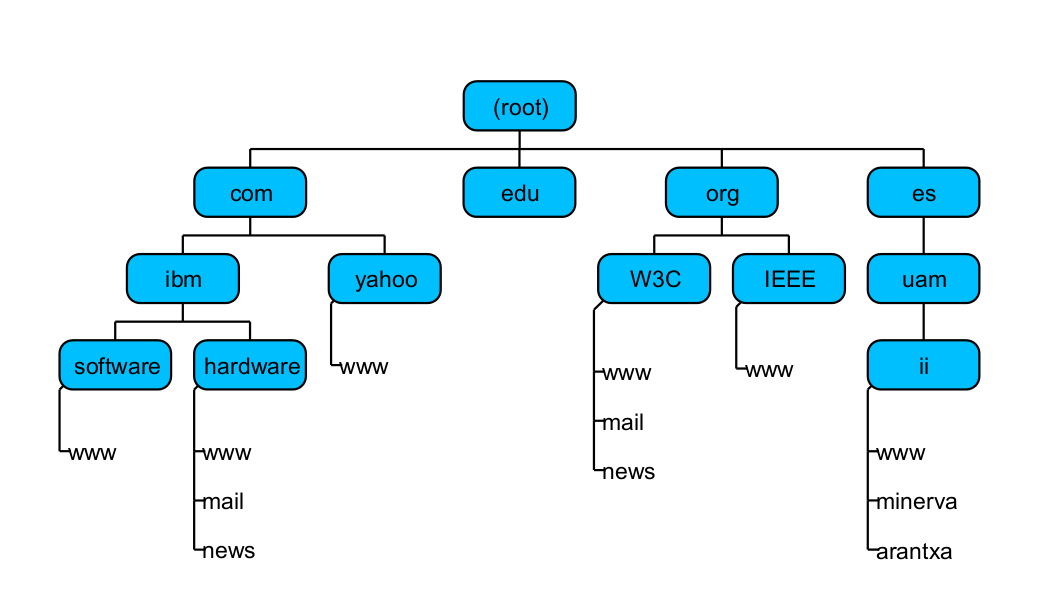
\includegraphics[width=1\textwidth]{img/namespaces.png}
\caption{Espacio de nombres jerárquico.}
\label{namespaces}
\end{figure}

Estos espacios de nombres se pueden utilizar también orientándolo a objetos, de tal manera que cada entrada es una instancia de un objeto. También se pueden tener distintas copias para cada dominio o distribuirlo organizándolo en servicios administrados separadamente ya que el acceso dentro de un dominio sólo requiere un nombre local.

\paragraph{Estándar \concept{X.500}}
Vamos a definir unas cuantas siglas\footnote{Por si acaso no llevamos ya suficientes} necesarias para explicar este estándar

\begin{defn}[XDS]
	APIs de X/Open Direcrory Service
\end{defn}

\begin{defn}[DUA]
	Directory User Agent
\end{defn}

\begin{defn}[DAP]
	Direcroty Access Protocol
\end{defn}

\begin{defn}[DSA]
	Directory System Agent
\end{defn}

\begin{defn}[DSP]
	Direcroty System Protocol
\end{defn}

Los clientes contienen el DUA y se comunicacn con los servidores utilizando DAP.

Los servidores contienen el DSA y se comunican entre servicores utilizando DSP.

Al directorio en sí se accede con las APIs de XDS.


\begin{figure}[hbtp]
\centering
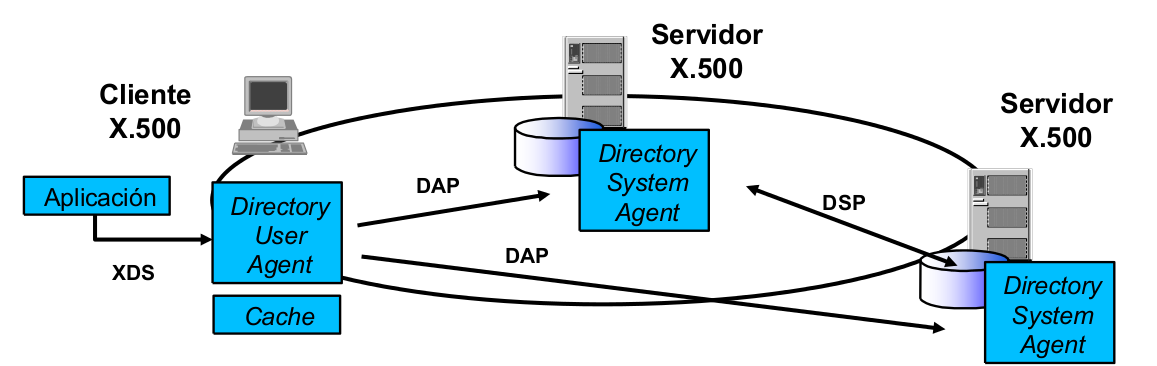
\includegraphics[width=1\textwidth]{img/X500.png}
\caption{Esquema de funcionamiento del estándar X.500.}
\label{X500}
\end{figure}

Existe una alternativa al DAP que es el \concept{LDAP} (\textit{Lightweigth Directory Access Protocol}). Este protocolo no requiere espefícicamente de un directorio X.500, puede utilizarse con \textit{Microsoft Active Directory}.

Esto es un protocolo de comunicaciones, no es una especificación de directorio ni una API de programación. No confundirse.


\subsection{Servicios de tiempo}

Es básico y fundamental que cuando tenemos un sistema distribuido todos los relojes estén perfectamente sincronizados. Para ello existen los servicios de tiempo que vamos a estudiar a continuación.

Sincronizar 2 personas sus relojes es fácil, porque los 2 ven en el mismo instante de tiempo los 2 relojes. 2 ordenadores separados no pueden ver los relojes a la vez, ya que el mensaje con la hora que tiene cada uno tarda en llegar, es por ello que cada ordenador \textbf{mantiene un componente de inexactitud} y que es necesario \textbf{sincronizar periódicamente} cuando ese componente de inexactitud supere un umbral definido\footnote{Tal vez nos podemos permitir 0.01 segundos de desincronización, pero no podemos permitirnos 0.05}

Mantener sincronizado el tiempo es imporescindible para la consistencia y para la \textbf{seguridad}.

Para lograr esta sincronización existen proveedores de tiempo (\concept{timer ticks}) que pueden sincronizar por radio      y actualizar el reloj del administrador de nuestro sistema distribuido. Podemos conectar más de un servidor a estos proveedores.

Una vez tenemos definidos los servidores de nuestro servicio con la hora buena (sincronizados con los timer ticks) el resto de nuestros servidores realizan consultas para sincronizar sus relojes. El formato utilizado es \concept{UTC} (Universal Time Coordinated) que cuenta desde el principio del calendario gregoriano.


\subsubsection{NTP}
¿Y cómo implementamos o utilizamos un servicio de tiempo? Con el \concept{NTP} \textit{Network Time Protocol}, que define una arquitectura para un servicio de tiempo y un protocolo para distribuir la información del tiempo.

\begin{itemize}
	\item Precisión en la sincronización a UTC.
	\item Fiabilidad
	\item Actualizaciones frecuentes (por lo que será necesario que sea resistente a alto nivel de carga)
\end{itemize}

La red de servidores está organizada jerárquicamente. El primer estrato recibe UTC de fuentes  físicas de tiempo (llamadas estrato 0 en wikipedia) y el estrato 2 sincroniza con los primeros. El resto de la red sincroniza con el estrato 2.

Veamos un ejemplo de los cálculos necesarios para sincronizar dos servidores.

\begin{example}
El esquema de la comunicación (intercambio de mensajes) entre los dos servidores que se van a sincronizar es:
\begin{center}
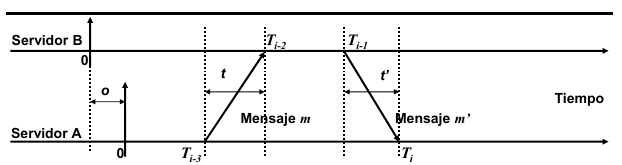
\includegraphics[width=1\textwidth]{img/ntp.png}
\end{center}

Nuestro objetivo es calcular $o$, que es la diferencia de tiempos entre ambos relojes. Observando el esquema, podemos deducir las ecuaciones:
\begin{align}
T_{i-3}+o+t=T_{i-2}\\
T_{i}+o=T_{i-1}+t'
\end{align}
Tampoco conocemos $t$ n $t'$, pues no sabemos el tiempo que ha tardado el mensaje en ser transmitido. Si sumamos las dos ecuaciones y despejamos $o$ de la nueva ecuación nos queda:
\[o=\underbrace{\frac{T_{i-2}+T_{i-1}-T_i-T_{i-3}}{2}}_{o_i}+\frac{t'-t}{2}\]

Así, tenemos $o$ escrito como la suma de un valor conocido más una desviación. Puesto que todos los tiempos son positivos, tenemos que $t+t'>t'-t$ por lo que podemos acotar $o$ mediante:
\[o_i-\frac{\overbrace{t'+t}^{d_i}}{2}\leq o \leq o_i + \frac{\overbrace{t'+t}^{d_i}}{2}\]
\end{example}

\subsection{Seguridad}
Aunque es un tema superimportante (porque en un sistema distribuido se complican las cosas) y tiene un tema dedicado explícitamente a esto, no se va a ver en este curso porque ...



\section{Problemas Tema 1}

  \begin{problem}[1]
  Diseñar, a nivel de bloques, un sistema por el cual un \textit{middleware} pudiera soportar redundancia en un servidor de archivos planos (tipo disco
  compartido) de modo transparente a la aplicación y los servidores
  que intervienen en la conexión.


  \solution



  \end{problem}

  \begin{problem}[2]
  Uno de los principales problemas que tiene que tratar cualquier
\textit{middleware} que comunique ordenadores de distinto tipo es la transparencia del formato
  de representación interno de los datos en cada componente de la
  red. Estudiar las ventajas e incovenientes de cada una de estas tres posibles
  alternativas en distintas situaciones de sistemas distribuidos:
    \begin{itemize}
    \item Convertir todos los datos al formato interno de uno de los componentes
    de la red.
    \item Convertir todos los datos a un formato intermedio de intercambio.
    \item No realizar ninguna conversión en el \textit{Middleware}, y dejar que cada
aplicación realice las conversiones que considere oportunas.
\end{itemize}
    \solution
\textcolor{green}{Dejuan opina que:}

Convertir todos los datos a un formato intermedio requiere que tanto el cliente como el servidor realicen una conversión. Si pensamos en términos de idiomas entre personas se entiende muy fácilmente. Si yo hablo ruso y tu chino, ¿para qué vamos a aprender los 2 español?

Mejor será que yo aprenda chino o tu ruso, es decir, convertir todos los datos al formato de uno de los componentes require menos trabajo (por lo menos a los componentes que no tienen que convertir nada).

En cuanto a no realizar ninguna conversión, la ventaja que presenta es que el middleware es un software más ligero porque tiene menos funciones, pero presenta la gran desventaja de que a los desarrolladores les obliga a conocer las representaciones internas de los datos de los componentes del sistema distribuido y les añade una complejidad innecesaria.

    \end{problem}

  \begin{problem}[3]
  En un sistema de comunicaciones mediante RPCs, estudiar el lugar adecuado
para introducir la función de conversión del formato de representación de los
datos descrita en el problema anterior. Nota: Basarse en la figura \ref{RPCimg}.
  \solution

\textcolor{green}{Dejuan opina que:}

Suponiendo que el formato elegido sea el del servidor, el cliente tendría que realizar el \textit{marshalling} al enviar un RPC en el momentos 2 (al enviar) y el \textit{unmarshalling} en el 10 (al recibir) de la imagen, cuando el \textit{Client stub} codifica y descodifica\footnote{tal vez codifica y descodifica no son las palabras adecuadas} respectivamente el mensaje para dárselo al nivel de transporte.

  \end{problem}

  \begin{problem}[4]
  Sugerir alguna alternativa al servicio \textit{portmapper} empleado en la
comunicación mediante RPCs para conocer la dirección (puerto) del servidor
con el que se desea comunicar, basado en alguno de los servicios que puede
desempeñar un \textit{middleware}.
  \solution

\textcolor{green}{Dejuan opina que:}


RM-ODP define que el NOS \ref{NOS} (una de las 3 capas del middleware) puede proporcionar transparencia ofreciendo un servicio de nombres y transparencia a la ubicación, movilidad y reubicación.

Si se definiera un espacio de nombres o se incluyera la funcionalidad de conocer los puertos en el NOS solucionaríamos la necesidad del \textit{portmapper}

  \end{problem}

  \begin{problem}[5]
  Un determinado sistema distribuido requiere que cada servidor autentique
  la conexión de sus clientes mediante la introducción de un
  identificador de usuario y una contraseña. Supuesto que posee un
  \textit{middleware} genérico, diseñar sobre él un servicio que permita a las
aplicaciones clientes realizar una validación única de usuario y contraseña,
independientemente del número de servicios que sea necesario utilizar.
  \solution

\textcolor{green}{Dejuan opina que:}


No entiendo bien la pregunta. Para diseñarlo en serio haría falta más información.

Por middleware genérico tampoco entiendo qué incluye. Una de las características deseables del NOS es \textit{Single Sign On, SSO}, un único usuario y contraseña para todos los servicios. Si el middleware genérico que tenemos incluye un NOS con SSO, entonces tendríamos que añadir la funcionalidad de permitir inicio de sesión distribuido, sabiendo que el usuario y la contraseña es la misma para todo el sistema.

\yoP

Entiendo que lo que piden es describir una arquitectura o procedimiento que te permita llevar a cabo esta tarea.

Suponiendo que tenemos un sistema con varios servidores, podemos hacer que uno de ellos sea el encargado de la autenticación de los usuarios. Una vez que este servidor comprueba que tienes permisos de acceso te devuelve un identificador y el mismo identificador codificado con su clave privada (a modo de firma).

Cada vez que el cliente conecte con alguno de los servidores, enviará este identificador junto con la firma con lo que el servidor destino sólo tendrá que coger su clave para comprobar que el cliente ya está loggeado.

Al margen de las claves que permitan relacionarse a un servidor con otro a través del cliente de modo seguro, serían necesarias más pares de claves de modo que la comunicación cliente-servidor también fuese segura.
  \end{problem}

  \begin{problem}[6]
  Partiendo del esquema de comunicación entre programas a través de la
interfaz \textit{socket} (\ref{SocketNoConexion}), ampliar el esquema correspondiente al programa servidor para que sea capaz de atender conexiones simultáneas de varios programas clientes.

Sugerencia: Utilizar una tarea en el servidor por cada conexión.
  \solution

\textcolor{green}{Dejuan opina que:}

La interfaz de socket a la que se refiere el enunciado (la de la página 12 de las transparencias) es socket no orientado a conexión.

Para poder atender simultáneamente conexiones, habría que crear hilos antes del \textit{rcvfrom()} para que atendieran a los diversos clientes.


  \end{problem}

  \begin{problem}[7]
  Un sistema de control de inventario central recibe los movimientos de
mercancía que se realizan en su red de almacenes, y de ellos debe ser capaz en
todo momento de conocer la cantidad de cada producto que existe en toda la red.
Proponer el mecanismo de comunicaciones que se considere más adecuado para
realizar estos envíos, considerando distintos casos:

    \ppart Todos los sistemas operan simultáneamente, y disponen de enlaces de
comunicaciones dedicados.
    \ppart Todos los sistemas operan simultáneamente, pero los enlaces de que disponen
son conmutados.
    \ppart Los sistemas tienen distinto horario de funcionamiento.

    \solution

    \yoP

    Entendemos que tenemos un sistema de varios servidores (conectados, obviamente, a muchos clientes pero eso no nos importa) y queremos que estén correctamente sincronizados estos servidores, de modo que si un cliente compra algo, el stock de todos se reduzca.

    \spart

    Si tienen enlaces de comunicación dedicados es posible que cada servidor informe al resto en tiempo real de todos los cambios que se experimentan, de modo que todos los servidores pudieran tener siempre información actualizada.

    \spart
    Si los enlaces son conmutados, al mandar un servidor un mensaje, el enlace queda bloqueado, por lo que una comunicación en tiempo real no sería viable. \textcolor{blue}{No se exactamente qué se debería hacer aquí}

    \spart

    Por definición, parece que lo óptimo es el empleo de una cola de mensajes donde los servidores informan de los cambios. Cuando un servidor arranque, antes de empezar a trabajar, actualiza su información en base a los mensajes de la cola.

    \end{problem}

  \begin{problem}[8]
  Nombrar casos de comunicación entre aplicaciones en los que sea
preferible emplear colas no persistentes en lugar de colas persistentes.
Razonar la respuesta.
  \solution

\textcolor{green}{Dejuan opina que:}

Recordamos que persistencia en colas significa que persistan los mensajes de la cola, no la cola en sí. (La persistencia de la cola se llama temporalidad).

Si eres el de misión imposible y quieres que los mensajes con la misión que mandas se autodestruyan, puede ser interesante implementar una cola no persistente.

\yoP

En general puede ser interesante cuando no te preocupe preservar o no los mensajes, puesto que hacer la cola persistente implica un coste extra que puedes ahorrar.

No creo que haya ningún momento en que te interese perder la información, simplemente puede darse el caso de que no rente el coste necesario para mantener esos mensajes en caso de fallo.


  \end{problem}

  \begin{problem}[9]
  Enumerar las ventajas e inconvenientes que puede tener sustituir un mecanismo
  de comunicación entre procesos interno de un sistema operativo (áeras
  de memoria compartidas, archivos, \textit{named pipes}, etc.) por colas locales
de \textit{MQSeries} para comunicar dos aplicaciones en el mismo ordenador.
Justificar brevemente cada una de ellas.
  \solution

  \yoP

  Para empezar es posible que no nos interese emplear colas de mensajes. Si necesitamos que una aplicación espere hasta que la otra finalice el proceso nos interesará emplear mecanismos de comunicación como los sockets en lugar de colas.

  Puestos a que nos interese el empleo de colas, las colas de MQSeries tienen el problema de que implican más carga de trabajo para el sistema operativo, pues en el fondo serán otro programa que se está ejecutando en el mismo host.

  Una posible ventaja del empleo de colas MQSeries es que, si tienen appis adecuadas para distintos lenguajes de programación, puede ser más sencilla la comunicación con ellas, pues las llamadas al sistema no son igual de sencillas en todos los lenguajes.

  Frente al empleo de áreas de memoria compartidas o sistemas de archivos, se tiene la ventaja de que las colas de mensajes, y en concreto las de MQSeries, permiten gestionar fácilmente el control de los mensajes leídos y los destinatarios de los mismos.


  \end{problem}

  \begin{problem}[10]
  Un sistema de directorio de nombres jerárquico consta de un nodo raíz, que
denominaremos A, y tres nodos secundarios que dependen de él, que denominaremos
B, C y D, respectivamente. No existe replicación de la información en ninguno
de los servidores de nombres de la estructura, de modo que cada servidor sólo
contiene la información de las estaciones que dependen de él. Expresar el flujo
de mensajes que debe tener lugar para que una estación del nodo B, que
denominaremos B1, pueda recuperar la información de directorio de una estación
dependiente del nodo C, denominada C1.
  \solution

  \yoP

  \begin{enumerate}
  \item[1] B1 pregunta a B por C1
  \item[2] B no conoce a C1 (sólo conoce a las estaciones que dependen de él), así que manda a B1 a preguntar a A, pasándole su dirección IP

  \item[3] B1 pregunta a A por C1 y A reconoce que estará asociado a C por que le envía a B1 la dirección de C. \textcolor{blue}{Dejuan opina que A debería preguntar a C y a D a ver de quién es C1, porque A sólo conoce los que dependen de Él, ¿no?}

  \textcolor{red}{Pedro manda a de Juan y a aquellos que tengan esta duda a mirar el ejercicio 20, que resolvió la profesora y en el que se observa que tu no buscas C1 a pelo sino que lo buscas conociendo su nombre completo. Es decir, estás buscando A.C.C1}

  \item[4] B1 pregunta a C por C1 y este, puesto que C1 depende de él, lo conoce y le dice a B1 la dirección de C1
  \item[5] B1 conecta con C1
  \end{enumerate}

  \end{problem}

  \begin{problem}[11]
  Determinar la tolerancia mínima de reloj que es necesario considerar
  debido a la propagación de la información por el medio físico en un sistema
  que sincronice desde un servidor de tiempo central los relojes de todas
  sus estaciones en los siguientes casos:
    \ppart Entorno de red de área local de un tamaño máximo de 500 m.
    \ppart Entorno de red de área extendida, máxima distancia de 600 Km.
    \ppart Entorno de red transoceánica por cable coaxial, máxima distancia entre
nodos de 10.000 Km.
    \ppart Red VSAT \textit{(Very Small Aperture Terminal}, red de comunicaciones vía
satélite) con nodo de retransmisión en un satélite en la órbita geoestacionaria
(36.000 Km. sobre el ecuador).
  \paragraph{Notas: }
  - Considerar la velocidad de propagación de un campo electromagnético
en un cable aproximadamente igual a 2/3 de la velocidad de la luz en el
vacío.

  - No se consideran efectos de elementos intermedios de la comunicación,
  ni a nivel físico (amplificadores,  regeneradores de señal) ni a niveles
  superiores (puentes o \textit{routers}).

  \solution

  \yoP

  Me niego a hacer los cálculos, hacemos cuentas para obtener el tiempo de transporte y atendiendo a las cuentas realizadas en el ejemplo \ref{ejemplo_tiempos}, vemos que la tolerancia mínima es $\pm\frac{t+t'}{2}$ donde $t$ y $t'$ son los tiempos de transporte del mensaje en ambas direcciones.

\textcolor{green}{Dejuan se anima a hacer las cuentas}

Recordamos que la velocidad de la luz es $c=3·10^8 m/s$, con lo que $v_p=2·10^8m/s$. 

\spart
\[
t = \frac{d}{v_p} = \frac{500m}{2·10^8m/s} = 2.5·10^{-6}  s
\]
\spart
\[
t = \frac{d}{v_p} = \frac{600Km}{2·10^8m/s} = 3·10^{-3} s
\]
\spart
\[
t = \frac{d}{v_p} = \frac{10^6m}{2·10^8m/s} = 5·10^{-2} s
\]
\spart
\[
t = \frac{d}{v_p} = \frac{36·10^6m}{2·10^8} =  1.8·10^{-1} s
\]
  \end{problem}

  \begin{problem}[12] A efectos de asignación de nombres a los distintos recursos
  que lo componen, un determinado sistema distribuido se encuentra dividido
  en distintos dominios administrativos, organizados de modo jerárquico
  según al esquema:

  \begin{center}
  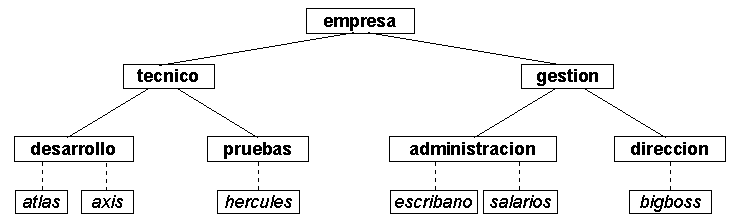
\includegraphics[width=1\textwidth]{img/si2-t4-ej-dom1.png}
  \label{Subnormalidad.}
  \end{center}

  Los nodos en cursiva representan ordenadores, y los nodos en negrita, los dominios.


  Cada dominio tiene un servidor de nombres propio, que reside en un ordenador
    cuyo nombre coincide con el del dominio, con capacidad de almacenamiento local
    de resultados de consultas a otros dominios (cache). Inicialmente se supone que
    todas las caches de los dominios se encuentran vacías.

    \ppart Poner los nombres completos en el dominio global de cada uno de los
      ordenadores representados en cursiva en la figura.
    \ppart Detallar los mensajes que serán necesarios y entre qué sistemas deben
        circular para que el ordenador atlas localice el servidor salarios en el
        directorio a partir de su nombre en la red.
      \ppart Inmediatamente después de la anterior consulta, el ordenador axis necesita
          establecer una conexión con salarios. Indicar el flujo de mensajes que ocurrirá
        para que pueda localizarlo en el directorio.
      \ppart Supuesto que el sistema de nombres que se emplea sigue el estándar X.500, nombrar:
            \begin{itemize}
              \item Ordenadores que contendrán un \textit{Directory User Agent}.
              \item Ordenadores que contendrán un \textit{Directory System Agent}.
              \item Tres parejas de ordenadores entre las que se empleará un \textit{Directory Access Protocol}.
              \item Tres parejas de ordenadores entre las que se empleará un \textit{Directory System Protocol}.
            \end{itemize}
      \ppart Proponer un sistema de comunicaciones (\textit{peer to peer} orientado a conexión, no orientado a conexión, \textit{Remote Procedure Calls},
 colas de mensajes) para producir los intercambios de mensajes de
resolución de nombres en el directorio, y razonar la respuesta.


\solution

\yoP

\spart

No pienso escribirlos todos. Es trivial. Por ejemplo, en el caso del host \textit{hércules} su nombre completo en el dominio global sería \textit{empresa/técnico/pruebas/hércules}

\spart

Equivalente al ejercicio 10.

\begin{enumerate}
\item[1] \textit{Atlas} pregunta a \textit{desarrollo} por \textit{salarios}
\item[2] \textit{Desarrollo} pregunta a \textit{técnico} por \textit{salarios}
\item[3] \textit{Técino} pregunta a \textit{empresa} por \textit{salarios}
\item[4] \textit{Empresa} pregunta a \textit{gestión} por \textit{salarios}
\item[5] \textit{Gestión} pregunta a \textit{administración} \textcolor{blue}{y a dirección (según Dejuan)} por \textit{salarios}
\item[6] \textit{Administración} envía a \textit{gestión} la dirección de \textit{salarios}
\item[7] El mensaje recorre la cadena en dirección contraria hasta llegar a \textit{atlas}
\end{enumerate}

\spart

Suponiendo que los servidores guardan en la caché información de las consultas recientes, el servidor \textit{desarrollo} ya tiene guardado en caché la dirección de \textit{salarios}, por lo que le responde directamente a \textit{axis}

\spart

\begin{itemize}
\item \textbf{Directory User Agent}:

Los que están en cursiva
\item \textbf{Directory System Agent}

Los que están en negrita
\item \textbf{Directory Acces Protocol}

\subitem axis-atlas
\subitem atlas-hércules
\subitem salarios-bigboss

\item \textbf{Directory System Protocol}
\subitem desarrollo-técinico
\subitem empresa-gestión
\subitem administración-dirección
\end{itemize}

\spart

La cola de mensajes no tiene sentido pues necesitamos obtener respuestas en tiempo real.

Peer to peer tampoco termina de encajar con la lógica del sistema, pues hay un claro comportamiento jerárquico y cada host pregunta de forma única a otro host y no pregunta a un tercero hasta no obtener su respuesta.

El método más interesante sería RPC donde cada host establece comunicación directa con aquel con el que quiere comunicarse. Además no tenemos que preocuparnos por la representación interna de los datos por lo que cada no podría estar programado en un lenguaje completamente diferente.

\textcolor{blue}{A Dejuan no le gusta RPC} porque no necesitamos ejecutar funciones que se encuentren en otros servidores, simplemente queremos hacer una pequeña consulta por lo que lo que más le convence es \textit{peer to peer} (porque no sólo hablas con el de arriba sino también con los que puedan tener debajo) y como no son muy frecuentes las consultas (debido a la caché) opina que lo ideal sería no orientado a conexión.

\end{problem}


  \begin{problem}[13]
  Se desea realizar un servidor para una red de área local que actúe como
punto focal de recepción de alarmas que se produzcan en las estaciones de
trabajo ante situaciones de diversos tipos (conexión de estación, fallos de
programas, errores en disco,introducciones de contraseñas equivocadas, etc.).

    \ppart Enumerar los mecanismos de comunicaciones que se pueden emplear para
enlazar los clientes con el servidor para realizar esta función u otras
similares.

    \ppart Valorar el empleo de cada uno de los mecanismos anteriores para realizar la
aplicación, y elegir la que se considere más apropiada a este caso, razonando
la respuesta.
    \ppart Si el prototipo de función que se desea utilizar en las estaciones clientes
para enviar una alerta es el siguiente:
\begin{verbnobox}[\small]
long alerta (
char tipo_alerta,      // Tipo de alerta que se ha producido
char nivel_gravedad,   // Nivel de gravedad de la misma
char * datos_adicionales,// Texto informativo dado por el cliente
long * codigo_accion   // Acción recomendada por el servidor
);                     //  para resolver la situación.
\end{verbnobox}
    en la que el valor que retorna la función indica si se ha completado
correctamente o no la función, tanto por motivos de la red como del servidor,
definir:
    \begin{itemize}
      \item Una estructura de mensaje apropiada para la comunicación entre cliente y
servidor.
      \item Explicar el proceso de \textit{Parameter Marshalling} que será necesario
realizar en el cliente antes del envío del mensaje. (Sugerencia: emplear C o
pseudocódigo, comentado).
      \item Explicar el proceso de \textit{Parameter Unmarshalling} que será necesario
realizar en el cliente al recibir el mensaje de contestación. (Igual sugerencia).
    \end{itemize}
      \solution

      \yoP

      \spart

      Puestos a enumerar tendríamos: WS, P2P, RPC y colas de mensajes como principales opciones. \textcolor{green}{Dejuan opina que} RPC no es un mecanismo de comunicación sino de ejecución de servicios remotos, con lo que no lo considera una opción. Por otro lado, dentro de WS no hay que olvidarse de una arquitectura REST.

      \spart

      Vamos a analizar cada posibilidad por separado

      \begin{itemize}
      \item \textbf{WS}

      Sería fácil de emplear pero bastante lento para la comunicación. Además requiere comunicación síncrona lo cual puede no ser demasiado interesante a la hora de que muchos servidores envíen mensajes a un único punto.


      \textcolor{green}{Dejuan opina que} no tiene mucho sentido utilizar un WS, ya que el servidor no ofrece ningún servicio, simplemente tiene que ser informado. Es por ello que aunque utilizáramos REST tiene poco sentido. Incluso aunque REST es muy útil en este caso ya que es válido para sistemas heterogéneos. Además, la comunicación sería muy sencilla basándonos en peticiones POST de HTTP. Esta opción si permitiría comunicación asíncrona.

      \item \textbf{P2P}

      No encaja con la idea del trabajo a desarrollar puesto que tenemos una clara jerarquía con un único nodo con el que nos queremos comunicar. Además fuerza a que todas las estaciones de servicio acuerden un mismo lenguaje, pues no está ideado para host heterogéneos.

      \item \textbf{RPC}

      Útil para trabajar con host heterogéneos pues el propio middleware se encargará del marshalling y unmarshalling. Establece conexión directa entre los dos hosts que se quieren comunicar.

      \item \textbf{Colas de mensajes}

      Independiente de la plataforma sobre la que se implemente cada estación de trabajo salvo por el formato de los mensajes, que se debe acordar previamente. Permite la comunicación asíncrona, cosa que no permitían ninguna de las anteriores opciones.

      \end{itemize}
    Puesto que queremos que cada estación de servicio envíe la alarma y siga trabajando en detectar posibles fallos y, presumiblemente, habrá diferentes categorías de alarmas, lo más interesante sería el empleo de \textbf{colas de mensajes} que ayudan a la organización jerárquica de los errores y evitan la saturación del ordenador central.

      \spart

      \begin{itemize}
        \item Basta con que el mensaje tenga 2 campos, cada uno de los cuales se corresponde a uno de los strings que forman parte de la alerta. El tipo del mensaje será el tipo de alerta y la prioridad será el nivel de gravedad.

        \item El marshalling será el proceso de escribir el mensaje a partir de una variable de tipo alerta.

        \item El unmarshalling será justo el proceso contrario, a partir de un mensaje se construye una variable de tipo alerta.
      \end{itemize}

      \end{problem}

  \begin{problem}[14]
  A continuación se presentan cuatro casos de sistemas servidores.
  \begin{enumerate}
    \item Servidor de archivos Unix para una red de ordenadores personales en MS-DOS.
    Los clientes deben ver el disco del servidor como si fuera un disco local.
    \item Servidor de envío diferido de fax. El servidor del que se dispone permite a
los clientes conectados a él a través de una red de comunicaciones enviar un
fax desde su estación, compartiendo una única línea de teléfono y aprovechando
las horas de menor coste de las llamadas telefónicas.
    \item Servidor de emulación de terminales. Permite a sistemas clientes
ASCII acceder al ordenador servidor, que trabaja con código EBCDIC, como si se
encontraran en una pantalla local del mismo.
    \item Servidor de validación de contraseñas para una red de ordenadores
homogénea. Recibirá un identificador de usuario y contraseña, debidamente
cifrados, y contestará al cliente únicamente si ambos son correctos, enviando un mensaje de reconocimiento.
  \end{enumerate}
  Para cada uno de ellos se pide:
  \begin{itemize}
    \item Elegir razonadamente el mecanismo de transporte (\textit{peer to peer} orientado a conexión, \textit{peer to peer }no orientado a conexión, RPCs, colas de menajes) que sería aconsejable utilizar para conectar a ellos los sistemas clientes.
    \item Indicar, si es necesario, las funciones adicionales que
habría que implementar sobre el protocolo elegido para garantizar que el
 \textit{middleware }resultante garantizara la transparencia de acceso del sistema distribuido.
  \end{itemize}
    \solution


    \begin{enumerate}
    \item

    Puesto que los ordenadores serán heterogéneos (ordenadores personales en MS-DOS pero servidor de archivos UNIX)  será necesario un proceso de marshalling y unmarshalling. Un único fichero puede estar repartido entre múltiples servidores pero los clientes no deben notarlo.

    Además necesitamos un acceso rápido y ligero, por lo que lo más interesante sería el uso de RPC.


    \item

    Puesto que el envío del fax no se realizará en el instante exacto en que se selecciona la opción sino que se aprovecharán las horas de menor coste de las llamadas telefónicas, lo más apropiado sería el empleo de una cola de mensajes.

    El cliente que quiera mandar un fax deja un mensaje en el servidor y este, cuando la línea esté desocupada, tomara un mensaje de la cola y enviará el fax pedido.

    \item

    Es necesaria comunicación fiable sin pérdida de paquetes o los comandos que se ejecuten podrían llegar incompletos dando lugar a resultados inesperados. Por tratarse de sistemas heterogéneos (unos emplean ASCII y otros EBCDIC) sería recomendable el uso de RPC que se encarga del unmarshalling y marshalling de manera transparente a los usuarios.

    \textcolor{red}{La solución de la profesora dice que no merece la pena el RPC puesto que la funcionalidad de traducción necesaria es muy sencilla. Por tanto emplean P2P orientada a conexión}

    \item

   Los dos sistemas tienen que estar conectados a la vez. La red es homogénea, luego no es necesario traducción de datos para garantizar transparencia de acceso.
   Puesto que la funcionaldiad es muy elemental no merece la pena RPC.

   Sólo tenemos un mensaje y una respuesta por lo que no merece la pena crear
   una conexión y las llamadas son síncronas.

  La solución más apropiada es comunicación P2P no orientada a conexión.

    \end{enumerate}

    \end{problem}



  \begin{problem}[15]
  Se desea construir un servidor de objetos distribuidos para
implementar un diccionario on-line con hipertexto. Cada palabra definida
 por el diccionario es un objeto. Los objetos están almacenados en
archivos. Cada archivo tiene una tabla con los nombres de los objetos
que contiene y un puntero al lugar donde está almacenado. Cada objeto
contiene información sobre su tamaño, los atributos que posee y los
tipos de datos correspondientes, que pueden ser:

\begin{enumerate}
  \item	Vectores de enteros

  \item	Vectores de strings.
\end{enumerate}
  
  El servidor asigna a cada cliente un hilo y se comunica con él mediante una tubería
  (pipe)
      \ppart ¿Qué operaciones posibles realizará el servidor, y qué información debe enviarle el cliente para solicitarlas?
    \ppart ¿Qué información debe devolver el servidor?
    \ppart Definir una estructura de mensajes adecuada, para que un objeto pase a través de la tubería.

 \solution

\yoP

\spart
Puesto que se trata de un diccionario on-line, el servidor deberá hacer las funciones de búsqueda de objetos a partir de su nombre.

\spart
Para cada palabra que se busque se deberán devolver los datos de dicha palabra.

\spart

Se pueden escribir los atributos del objeto separados por el símbolo ';'. Para los vectores separamos cada elemento del siguiente mediante una coma, ',' y un vector del otro con ';'

 \end{problem}



  \begin{problem}[16]
  (Coulouris 10.7) Un servidor B de NTP recibe un mensaje del servidor A
  a las 16:34:23.480 llevando una marca de tiempo 16:34:13:430 y lo responde.
  A recibe el mensaje a las 16:34:15.725, llevando una marca de tiempo 16:34:25.7
  de B. Estimar la deriva entre B y A y la precisión de la estimación.
  \solution

  \yoP

  El esquema que tenemos para el ejercicio es el que hemos visto en teoría:

  \begin{center}
  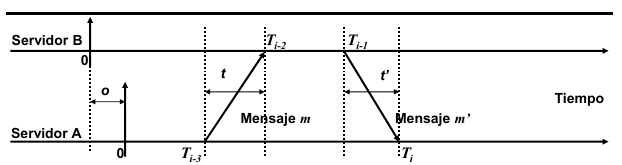
\includegraphics[width=1\textwidth]{img/ntp.png}
  \end{center}

Con la misma nomenclatura de la imagen tenemos:

  \[\left\{ \begin{align}
T_{i-3}&=430 \\
T_{i-2}&=10050\\
T_{i-1}&= 12270\\
T_{i}&=2995
\end{align}
\right.\]

donde los tiempos los hemos tomado midiendo desde las 16:34:13, para hacer los números más pequeños y manejables (trabajando en milisegundos). \textcolor{green}{Hay una pequeña errata: $T_{i-2}=10480$ porque medimos desde 16:34:13 y para que fuera 10050 tendríamos que estar midiendo desde 16:34:13:430}

Nuestro objetivo es calcular $o$, que es la diferencia de tiempos entre ambos relojes. Observando el esquema, podemos deducir las ecuaciones:
\begin{align}
T_{i-3}+o+t=T_{i-2}\\
T_{i}+o=T_{i-1}+t'
\end{align}
Tampoco conocemos $t$ n $t'$, pues no sabemos el tiempo que ha tardado el mensaje en ser transmitido. Si sumamos las dos ecuaciones y despejamos $o$ de la nueva ecuación nos queda:
\[o=\underbrace{\frac{T_{i-2}+T_{i-1}-T_i-T_{i-3}}{2}}_{o_i}+\frac{t'-t}{2}\]

Así, tenemos $o$ escrito como la suma de un valor conocido más una desviación. Puesto que todos los tiempos son positivos, tenemos que $t+t'>t'-t$ por lo que podemos acotar $o$ mediante:
\[o_i-\frac{\overbrace{t'+t}^{d_i}}{2}\leq o \leq o_i + \frac{\overbrace{t'+t}^{d_i}}{2}\]

Así, podemos decir que la deriva es: $o_i=9447.5ms$ con una precisión de $\pm 172.5 ms\footnote{Para obtener t'+t restamos las dos ecuaciones del sistema}$


  \end{problem}

  \begin{problem}[17]
  Los protocolos de comunicaciones pueden ser orientados a conexión o no
  orientados a conexión. Describir los pros y los contras de cada uno de
  ellos para su utilización como medio de transporte de un sistema distribuido,
  e identificar el tipo más adecuado para realizar accesos a un servidor
  iterativo o a un servidor concurrente.
  \solution
\begin{itemize}
\item \textbf{Orientado a conexión: TCP}

 \subitem \textbf{Ventajas:}
 \begin{itemize}
\item Confiable: se garantiza recepción del mensaje.
\item Garantiza entrega de mensajes en el orden correcto.
\item Incorpora control de flujo.
\item No hay límite en el tamaño de los mensajes.
\end{itemize}
\subitem \textbf{Desventajas:}
\begin{itemize}
\item Mayor sobrecarga de procesamiento (mantener conexión).
\item Mayor información de protocolo en las cabeceras.
\item Limitado a la comunicación 1 a 1.
\end{itemize}

\item \textbf{No orientado a conexión: UDP}
\end{itemize}
 \subitem \textbf{Ventajas:}
 \begin{itemize}
\item Comunicación 1 a N utilizando broadcast y multicast.
\item Menos sobrecarga (no hay que mantener conexión).
\item Menor información de protocolo en las cabeceras.
\end{itemize}
\subitem \textbf{Desventajas:}
\begin{itemize}
\item No hay información sobre mensajes consecutivos.
\item Posible pérdida de mensajes o duplicidad de los mismos.
\item Mensajes de tamaño limitado.
\item No hay control de flujo.
\end{itemize}

Una vez hemos analizado estas ventajas e inconvenientes de ambos protocolos, podemos decidir cuál de ellos es más ventajoso utilizar en cada uno de los casos planteados:

\begin{itemize}
\item \textbf{Servidor Concurrente:}
\begin{itemize}
\item Generalmente utilizan protocolos orientados a conexión.
\item Cuando se recibe una nueva petición de conexión se crea un
nuevo proceso o hilo que se encargará de gestionarla.
\item Ejemplos: servidores web (HTTP), servidores de acceso
remoto (Telnet), servidores FTP.
\item Excepciones: servidor TFTP (usa protocolo UDP)
\end{itemize}
\item \textbf{Servidor Iterativo:}
\begin{itemize}
\item Generalmente utilizan protocolos NO orientados a conexión.
\item Servidores del tipo petición / respuesta que no almacenan
estado.
\item Ejemplos: servidores DNS o servidores DHCP.
\item Excepciones: servidor Daytime (utiliza protocolo TCP).
\end{itemize}
\end{itemize}
  \end{problem}

  \begin{problem}[18]
  Los servidores de un sistema distribuido pueden ser de dos tipos: sin estado
  \textit{(stateless)}, es decir, que no recuerdan la historia de peticiones anteriores realizadas
  por el cliente; o con estado \textit{(statefull)}, en caso contrario. Identificar el tipo de protocolo de transporte más
  adecuado (orientado o no orientado a conexión) para realizar los accesos
  a cada uno de estos tipos de servidores.
  \solution

  Para los servidores \textbf{statefull}, por su facilidad para identificar mensajes consecutivos de un mismo cliente, son
más apropiados los \textbf{protocolos orientados a conexión}. Si se usasen protocolos no orientados a conexión habría que incluir un campo adicional en cada mensaje para asociarlos a un mismo cliente.

No obstante, existen algunas excepciones, como DHCP que utiliza UDP pero guarda un estado asociado a cada cliente (qué dirección IP tiene asignada)

 Los servidores \textbf{stateless} no guardan información alguna asociada a cada cliente. Generalmente son del tipo petición respuesta donde no se guarda información asociada a cada cliente ni importa el orden de los mensajes enviados.

 Un ejemplo son los servidores DNS, servidores web o NTP. Un cliente solicita una
pagina web, sin importar qué páginas web ha solicitado anteriormente. Ya que no hace falta identificar mensajes consecutivos de un mismo cliente son más apropiados los \textbf{protocolos no orientados a conexión} como UDP pues tienen menos sobrecarga.

Como en todo dentro de la informática existen expeciciones como son los servidores web o los servidores web que utilizan TCP, probablemente debido a la limitación en el tamaño del mensaje en
UDP.
  \end{problem}

  \begin{problem}[19]
  Un servicio de autenticación en una red de área local funciona
mediante un mecanismo de comunicación basado en Remote Procedure Calls,
RPCs genéricas. Dispone de las siguientes funciones:
  \begin{itemize}
    \item Autenticación de usuario: Recibe como parámetros un
identificador de usuario y su contraseña, y devuelve un código de
retorno 0 si usuario y contraseña son correctos, y -1 en caso contrario.
    \item Cambio de contraseña: Recibe como parámetros un
identificador de usuario, su contraseña actual y la nueva contraseña que
 se desea registrar. Devuelve un código de retorno 0 si se ha realizado
correctamente la actualización, y -1 en caso contrario.
    \item Obtención de lista de privilegios asociados a un usuario: Recibe como parámetro
    un identificador de usuario. Si dicho usuario existe en el sistema, devuelve
    un código de retorno 0 y dos listas de longitud variable: la primera con
    todos los atributos definidos en el sistema para el usuario, separados
    por espacios; y la segunda con los nombres de todos los servidores de la
    red a los que tiene acceso, también separados por espacios. Si el usuario
    no existe, devuelve un código de retorno -1.
  \end{itemize}
  Los identificadores de usuario, contraseñas, atributos de usuario y nombres
  de servidores son cadenas de caracteres ASCII que tienen un tamaño máximo
  de 16 caracteres.
  \begin{itemize}
    \item Suponiendo que la red es homogénea (el mismo tipo de sistema
para clientes y servidor), proponer una estructura de mensaje de
petición y una estructura de mensaje de respuesta para la comunicación
entre client stub y server stub adecuado a las tres RPCs. (Describir la
estructura en pseudocódigo o en lenguaje C, de modo que quede
suficientemente clara).
    \item Introducir los cambios necesarios en el mensaje de petición
 de la RPC de autenticación de usuario para soportar una red no
homogénea (clientes y servidor de distintos tipos).
    \item Comentar los problemas de seguridad que presenta el diseño
elegido para esta aplicación, y proponer alternativas para resolverlo.
     \end{itemize}
  \solution

  Olakase

  \end{problem}

  \begin{problem}[20]
  Los ordenadores de una empresa están conectados siguiendo el modelo cliente
servidor, de acuerdo con la siguiente organización jerárquica de dominios
administrativos:
\begin{center}
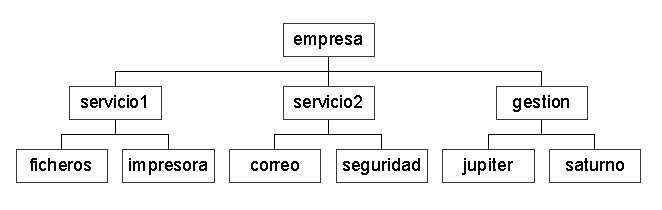
\includegraphics[width=1\textwidth]{img/si2-t4-ej-dom2.png}
\end{center}

   Las hojas del árbol representan ordenadores, los restantes nodos
dominios. Cada dominio tiene un servidor de nombres que reside en un
ordenador, cuyo nombre coincide con el del dominio, con capacidad de
almacenamiento local de resultados de consultas a otros dominios \textit{(cache)}. Se supone que al principio las caches están todas vacías.

    \ppart Escribir los nombres completos en el dominio global de todos los ordenadores
    situados en las hojas del árbol.
    \ppart Detallar los mensajes necesarios para que el ordenador jupiter localice
    el servidor seguridad en el directorio a partir de su nombre en la red.
    \ppart Inmediatamente después de la consulta anterior, el
ordenador saturno desea localizar el servidor seguridad. Indicar el
flujo de mensajes correspondiente.
    \ppart Suponemos que el sistema de nombres utiliza el estándar X500. Decir qué ordenadores contienen un \textit{Directory User Agent} y cuáles contienen un \textit{Directory System Agent}.
    \ppart Escribir tres parejas de ordenadores entre los que se utilice el \textit{Directory Access Protocol}.
    \ppart Escribir tres parejas de ordenadores entre los que se utilice el \textit{Directory System Protocol}.
    \ppart Para cada uno de los cuatro servidores (ficheros,
impresora, correo y seguridad) elegir razonadamente el mecanismo de
transporte aconsejable para conectar a ellos los ordenadores clientes:
peer to peer orientado a conexión, peer to peer no orientado a conexión,
 RPC o MOM.

\solution

\spart
\begin{itemize}
\item ficheros.servicio1.empresa
\item impresora.servicio1.empresa
\item correo.servicio2.empresa
\item seguridad.servicio2.empresa
\item jupiter.gestion.empresa
\item saturno.gestion.empresa
\end{itemize}

\spart
\begin{center}
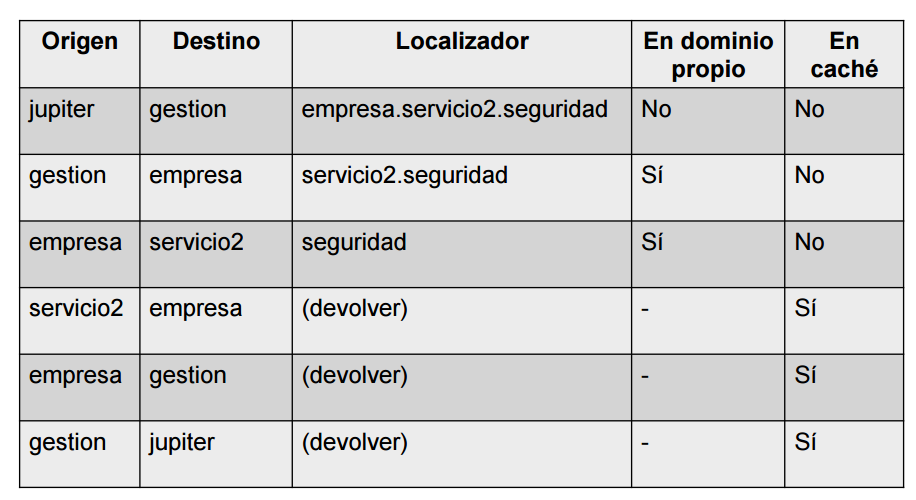
\includegraphics[width=1\textwidth]{img/H2_E20_B.png}
\end{center}

\spart
\begin{center}
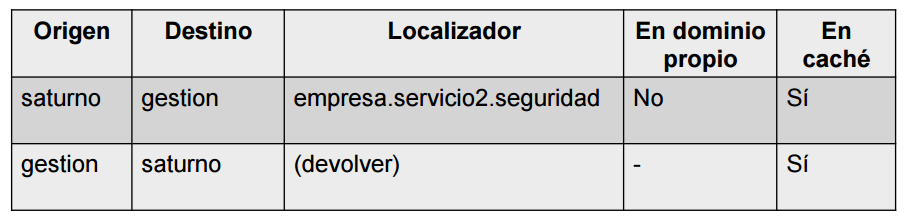
\includegraphics[width=1\textwidth]{img/H2_E20_C.png}
\end{center}

\spart
\begin{itemize}
\item \textbf{Directory User Agent}

ficheros, impresora, correo, seguridad, jupiter, saturno
\item \textbf{Directory System Agent}

empresa, servicio1, servicio2, gestion
\end{itemize}

\spart

\begin{itemize}
\item fichero – servicio1
\item correo – servicio2
\item seguridad – gestion
\end{itemize}

\spart
\begin{itemize}
\item servicio1 – empresa
\item servicio2 – empresa
\item gestion – empresa
\end{itemize}

\spart

\yoP

TO BE CONTINUED...

Me da mucha pereza y no estoy seguro de lo que quieren pero creo que habría que pensar que para la impresora nos interesa cola de mensajes, para el correo igual, para la parte de seguridad posiblemente necesitemos RTP, para la de ficheros TCP si es sólo escritura directa, o incluso UDP y para la parte de gestión pues no sabemos nada porque no tenemos detalles.
\end{problem}

\chapter{Colas}
\section{Teoría}
\section{Problemas Tema 2}
% -*- root: ../SI2.tex -*-



\chapter{Aspectos operacionales de los sistemas distribuidos: Disponibilidad}
\section{Introducción}
A lo largo de este tema vamos a estudiar la teoría de la disponibilidad de los sistemas distribuídos así como algunas arquitecturas que permiten obtener un incremento de la misma.

Para empezar debemos definir qué es la disponibilidad.

\begin{defn}[Disponibilidad]
La disponibilidad de un sistema es la probabilidad de que este se encuentre operativo en un instante de tiempo determinado.
\end{defn}

Hay dos motivos por los que un sistema puede no estar disponible:
\begin{enumerate}
\item[1] \textbf{Paradas no planificadas}

Este tipo de paradas se deben a fallos en los equipos o en los programas que implementan los servicios.

Requieren tratamiento estadístico, pues no habrá dos iguales. Los sistemas que las minimizan se llaman de \textbf{Alta Disponibilidad} \textit{(High Availability, HA)}


Algunas de las causas más frecuentes por las que se producen este tipo de paradas son:

\begin{itemize}
\item Extensión del tiempo destinado a operaciones planificadas.
\item Error humano.
\item Fallo en aplicación.
\item Fallo del sistema operativo.
\item Fallo hardware.
\item Errores de configuración del software.
\end{itemize}

\item[2] \textbf{Paradas planificadas}

Son requeridas por la aplicación para su correcto funcionamiento: Rearranques programados, copias de seguridad, cambios de configuración...

Por ser previsibles permiten un tratamiento sistemático. Los sistemas que las minimizan se denominan de \textbf{Operación Continua} \textit{(Continuous Operation, CO)}

Algunas de las causas más frecuentes por las que se producen este tipo de paradas son:

\begin{itemize}
\item Copias de seguridad.
\item Reemplazar o actualizar hardware.
\item Reemplazar o actualizar aplicaciones.
\item Actualizar sistema operativo.
\item Instalación de parches
\end{itemize}
\end{enumerate}

Evidentemente, un sistema ideal sería de Alta Disponibilidad y de Operación Continua. No obstante, a mayor disponibilidad del sistema mayor es el coste del mismo y su mantenimiento. Por tanto, es necesario valorar el nivel de disponibilidad requerido para un funcionamiento aceptable e invertir lo necesario para conseguirlo sin tratar de superarlo.

Antes de seguir estudiando el tema de la disponibilidad, vamos a ver una serie de definiciones de términos que aparecerán a lo largo de los apuntes y que es necesario precisar.

\begin{defn}[Fiabilidad (Reliability)][Fiabilidad]\index{Reliability}
Probabilidad de que un componente o sistema continúe funcionando en un determinado instante en el tiempo.
\end{defn}

\begin{defn}[Elasticidad o Resiliencia (Resiliency)][Resiliencia]\index{Elasticidad}\index{Resiliency}
Capacidad de un sistema para adaptarse a
condiciones externas imprevistas (fallos, aumento de carga...) para continuar cumpliendo sus parámetros de calidad.
\end{defn}

\begin{defn}[Mantenibilidad (Serviceability)][Mantenibilidad]\index{Serviceability}
Es la probabilidad de realizar una reparación satisfactoria en un tiempo determinado.
\end{defn}

\begin{defn}[Sistemas\IS tolerantes a fallos (Fault-Tolerant Systems)][Sistemas\IS tolerantes a fallos]
Sistemas que contienen
componentes hardware dobles de modo que el fallo de uno de ellos no suspende su
operación.
\end{defn}
\newpage
\begin{defn}[Clusters\IS de alta disponibilidad (High Availability Clusters)][Clusters\IS de alta disponibilidad]
Conjunto de nodos de servicio que comparten conexiones externas (red, discos...) y están gestionados por un software especial que permite proporcionar servicio sin interrupciones ante el fallo de alguno de sus componentes.
\end{defn}

\begin{defn}[Clusters\IS de alto rendimiento (High Performance Clusters)][Clusters\IS de alto rendimiento]
Conjunto de nodos de servicio que comparten una misma carga de trabajo.
\end{defn}

\begin{defn}[Recuperación ante desastres (Disaster Recovery)][Recuperación\IS ante desastres]
Capacidad de una instalación de
recuperar la operatividad tras un evento de gran magnitud, bien de tipo local (edificio), urbano (ciudad) o regional (área extendida con infraestructuras comunes).
\end{defn}

\section{Teoría de la disponibilidad}
\subsection{Disponibilidad}
La disponibilidad, $A$, de un sistema se estima a partir de la medida del tiempo que ha estado operativo, $T_{op}$, en un intervalo de tiempo, $T_{tot}$, suficientemente grande.
\[A= \frac{T_{op}}{T_{tot}}\]

Pero esta medida no da una idea global de la disponibilidad del sistema, pues un mismo valor puede obtenerse de la misma forma.

Por ejemplo, no es lo mismo que un sistema esté disponible 99 horas de cada 100 que 99 segundos de cada 100. Incluso si dos datos se han obtenido dividiendo los datos en las mismas unidades y estamos, por ejemplo, en 99 horas de cada 100 de actividad, puede ser que el sistema haya fallado una única vez en esas 99 horas y tardase una hora en recuperarse o que el sistema falle cada media hora tardando poco en recuperarse.

Por ello se utilizan otras medidas para estudiar la disponibilidad del sistema.

\begin{defn}[Tiempo medio\IS entre fallos]

En inglés \textbf{Mean Time Between Failures, MTBF}, es valor esperado del tiempo que transcurre entre dos fallos consecutivos de un equipo.
\end{defn}

\begin{defn}[Tiempo medio\IS hasta el fallo]

En inglés \textbf{Mean Time To Failure, MTTF}, es el valor esperado del tiempo de vida de un equipo o sistema, medida de su Fiabilidad (Reliability).
\end{defn}

\begin{defn}[Tiempo medio\IS de reparación/recuperación]

En inglés \textbf{Mean Time To Repair/Restore, MTTR}, es el valor esperado del tiempo que se tarda en sustituir un equipo averiado o recuperar un fallo de software.
\end{defn}

A partir de estos valores se calcula la disponibilidad según la fórmula:

\[A=\frac{MTTF}{MTBF}=\frac{MTTF}{MTTF+MTTR}\]

Para pasar de la primera a la segunda fórmula se emplea la relación lógica $MTBF=MTTF+MTTR$, es decir, el tiempo que transcurre entre dos fallos es la suma del tiempo que tarda en recuperarse el sistema tras un fallo más el tiempo que tarda en volver a fallar.

\subsection{Fiabilidad}

La fiabilidad de un componente o sistema en el tiempo es la probabilidad de que el sistema continúe funcionando en un instante de tiempo. Si denominamos $T$ al tiempo de vida del componente, su fiabilidad viene dada por la expresión:
\[R(t)=\mathbb{P}\{T > t \}\]

La vida del componente, $T$, es una variable aleatoria, cuya función de distribución es
\[F_T(t)=\mathbb{P}\{T \leq t \}\]

Evidentemente ambas variables probabilidades deben sumar siempre 1, $R(t)+F_T(t)=1$ y derivando obtenemos que sus funciones de densidad son iguales pero de signo contrario.

Una vez hemos definido estas variables podemos definir el tiempo medio hasta fallo como la esperanza de vida de un componente:
\[MTTF = E[T]=\int_{-\infty}^{\infty}fF'_T(t)dt\]

Ahora, sabiendo algo de probabilidad, podemos calcular la probabilidad de que un sistema falle antes de un instante, $x$, sabiendo que funcionaba en un instante $t<x$.
\[F_T(x | T > t ) = \mathbb{P}\{T \leq x | T> t\}=\frac{\mathbb{P}\{(T \leq x) \cap (T > t)\}}{\mathbb{P}\{T > t\}}=\frac{\mathbb{P}\{t < T \leq x\}}{\mathbb{P}\{T > t\}}=\]
\[=\frac{F_T(x)-F_T(t)}{1-F_T(t)}\]

y derivando con respecto a $x$ se obtiene
\[f_T(x | T > t)=\frac{f_T(x)}{1-F_T(x)}\]

A partir de esta última expresión se define la \concept{función de tasa de fallo} al evaluarla en $x=t$.
\[r(t)=f_T(t | T > t)=\frac{-R'(t)}{R(t)}\]

y se interpreta como la probabilidad de que un componente que funciona falle en el instante siguiente:
\[\mathbb{P}\{t<T\leq t + dt | T > t\}=f_T(t | T > t)dt=r(t)dt\]

Si la tasa de fallos tiene un valor constante, integrando la función $r(t)$ entre $0$ y $t$ y despejando $R(t)$ llegamos a:
\[R(t)=e^{-λt} \implies F_T(t) = 1-e^{-λt}\]

con lo que acabamos de obtener que el tiempo de vida es una distribución exponencial y su valor esperado será el MTTF=1/λ

\subsection{Distribución de los fallos}

La función de tasa de fallos en un equipo tiene la forma que se muestra en la figura:
\begin{center}
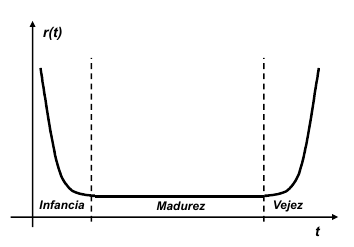
\includegraphics[width=0.7\linewidth]{img/tasa_fallos.png}
\end{center}

Durante la zona de infancia la tasa de fallos es alta debido al montaje de componentes defectuosos. Esta tasa de fallos se reduce con el tiempo hasta alcanzar una etapa de madurez que se correspondería con la época en que tenemos tasa de fallos constante. Por último el envejecimiento del equipo aumenta la tasa de fallos.

Todos los cálculos se realizan pensando en la zona de madurez del equipo, trabajando con $r(t)=cte$

Por otro lado tenemos también los fallos en programas que pueden dividirse en dos tipos según su tratamiento
\begin{enumerate}
\item[1] Programas que no son reparados cuando se encuentra el fallo sino que es necesario esperar a que se publique una nueva versión del mismo. Es la situación habitual en producción y con programas cerrados.

El modelo de tasa de fallos constante es válido durante el uso de una misma versión. Al cambiarla es necesario recalcular todos los datos.

\item[2] Programas cuyos defectos se corrigen conforme se encuentran. Suele tratarse de programas de producción propia o ciclos de pruebas en la producción de programas. El principal problema es que la solución de un defecto puede y suele introducir otros nuevos.

En este caso el modelo de tasa de fallos constante no es válido ya que tendremos una tasa de fallos que decrece con el tiempo (según se van arreglando los desperfectos). Su forma depende del modelo elegido para el ritmo de descubrimiento de fallos.

\end{enumerate}

\subsection{Mantenibilidad}
Es la probabilidad de realizar una reparación satisfactoria en un tiempo determinado. Mide la rapidez y facilidad con que un sistema se vuelve a poner operativo tras un fallo.
\[M(t)=\mathbb{P}\{T'> t\} \text{ con T' el tiempo de reparación}\]

Este tiempo incluye el tiempo necesario para descubrir el fallo, encontrar la causa, conseguir las piezas necesarias, la instalación de las mismas, arrancar el sistema de nuevo, etc. Es decir, incluye todo el tiempo gastado desde que \textbf{se produce} el fallo (aún si no se detecta) hasta que se resuelve el problema.

\[MTTR=E[T']\]

\subsection{Componentes en serie vs Componentes en paralelo}

Si tenemos un sistema compuesto por componentes en serie, un fallo en cualquiera de ellos implica un fallo global. La conexión en serie puede no ser física pero si lógica, una componente depende del resultado del trabajo de otra.

Suponiendo que el fallo en cada componente es independiende del resto, tenemos:
\[A= \prod_{i=1}^{n}A_i; \ \ \; R(t)=\prod_{i=1}^{n}R_i(t); \  \ \; r(t)=\sum_{i=1}^{n}r_i(t)\footnote{No veo clara esta fórmula}\]

Si tenemos un sistema compuesto por componentes en paralelo y estas componentes son redundantes para su funcionamiento, un fallo en una de ellas no implicará un fallo en el sistema.

Suponiendo que el fallo en cada componente es independiente nos queda:
\[A= 1-\prod_{i=1}^{n}(1-A_i)\footnote{Estará disponible cuando al menos una componente esté disponible}; \ \ \; F_T(t)=\prod_{i=1}^{n}F_{T_i}(t); \  \ \; R(t)= 1-\prod_{i=1}^{n}(1-R_i(t))\]

\begin{center}
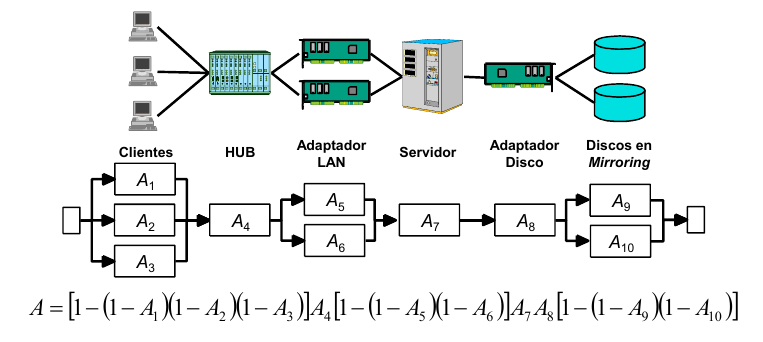
\includegraphics[width=\linewidth]{img/disponibilidad.png}
\end{center}



\section{Mejoras de la disponibilidad}

Recordemos la ecuación inicial que dimos para la disponibilidad:
\[A=\frac{MTTF}{MTTF+MTTR}=\frac{1}{1+MTTR/MTTF}\]

simplemente viendo esta fracción podemos ver que la disponibilidad de un sistema puede mejorarse (aumentar) de dos formas:
\begin{itemize}
\item Aumentando $MTTF$ mejorando la calidad de los equipos, introduciendo redundancias o eliminando \textbf{Puntos Simples de Fallo}

\item Reduciendo $MTTR$ mediante la reducción del tiempo empleado en cualquiera de las siguientes fases:
\begin{itemize}
\item Tiempo de \textbf{latencia} (desde que se da el fallo hasta que se descubre que algo falla)

\item Tiempo para aislarla (desde que se descubre hasta que se encuentra el motivo)

\item Tiempo para corregirla

\item Tiempo para verificar que todo funciona bien
\end{itemize}
\end{itemize}

\subsection{Arquitecturas que incrementan la disponibilidad}

La disponibilidad de una cadena de procesamiento es siempre menor que la menor de las disponibilidades de sus componentes. Denominamos \concept{Single Point Of Failure, SPOF} a los puntos más criticos del sistema, aquellos que al fallar implican la caída del servicio.

Como es evidente, la forma en que más podemos incrementar el $MTTF$ de cada componente es mediante la creación de un \textbf{cluster} (elementos redundantes) en cada parte de la cadena de procesamiento. Esta solución, además, elimina los SPOF al añadir redundancias incluso a esos componentes más críticos.

Conseguir que varios sistemas realicen en paralelo una misma función no es sencillo y la solución empleada depende de factores como el tipo de elemento al que se le quiere dar redundancia y las necesidades de disponibilidad del sistema completo.

En cualquier caso, siempre es necesario considerar dos procesos a la hora de implementar un sistema: el cómo actuar cuando se produce un fallo para poder mantener el servicio, \concept{Fail-over}, y cómo actuar para recuperar la situación normal una vez se resuelve el fallo \concept{Fail-back}.

Existen diferentes tipos de redundancia:
\begin{enumerate}
\item[1] \textbf{Según el estado de cada elemento del cluster}

Pueden estar todos los elementos activos (AA), uno activo y el resto preparados para activarse casi instantáneamente (AS) o uno activo y el resto detenidos pudiendo activarse en un cierto periodo de tiempo (AP)

\item[2] \textbf{Según el reparto de carga entre los elementos del cluster}

Puede ser dinámico (D), en cuyo caso no habrá que preocuparse en caso de fallo de un componente; o estático (E), donde un fallo implica reconfigurar el reparto de carga

\item[3] \textbf{Según el tratamiento de las conexiones activas}

Las sesiones activas pueden continuar (C) tras un fallo o ser interrumpidas (I).
\end{enumerate}

\section{Redundancia en los sistemas de comunicaciones}
Los sistemas de comunicaciones son uno de los puntos críticos de todo sistema distribuido.

Vamos a distinguir la redundancia en las redes de área local (LAN) y en redes de área extendida (WAN) considerando en ambos casos los estándares de facto actuales: redes LAN basadas en Ethernet y TCP/IP como medio de transporte.

Las características de los equipos que actualmente se emplean para implementar una LAN hacen que estas redes se puedan construir atendiendo a tres modelos distintos:
\begin{itemize}
\item \textbf{Nivel 2 compartido} Múltiples servidores se conectan a un mismo segmento de LAN implementado en un \textit{Hub}. Es el menos utilizado por ser el menos eficiente y flexible.

El hub es un dispositivo que tiene la función de interconectar las computadoras de una red local. Su funcionamiento es más simple comparado con el Switch y el router:
El hub recibe datos procedentes de una computadora, los transmite a los demás. En el momento en que esto ocurre, ninguna otra conmutadora puede enviar una señal. Su liberación surge después que la señal anterior haya sido completamente distribuida.


\item \textbf{Nivel 2 conmutado} Cada enlace es un segmento de LAN. Todos los componentes se interconectan mediante \textit{switches}, que actúan como puentes multipuerta.

Suele emplearse en el \textbf{nivel de acceso}, por ejemplo, en las conexiones de los ordenadores de las granjas de servidores.

\item \textbf{Nivel 3} Cada enlace es un segmento de red que une un elemento con un \textit{router}. El \textit{router} se implementa también en los propios \textit{switches} mediante módulos especiales.

Suele emplearse en el \textbf{nivel de agregación} interconectando diversos niveles de acceso, servidores especiales y redes externas.
\end{itemize}

Estos modelos suelen coexistir dentro de un Centro de Proceso de Datos (CPD)
\begin{center}
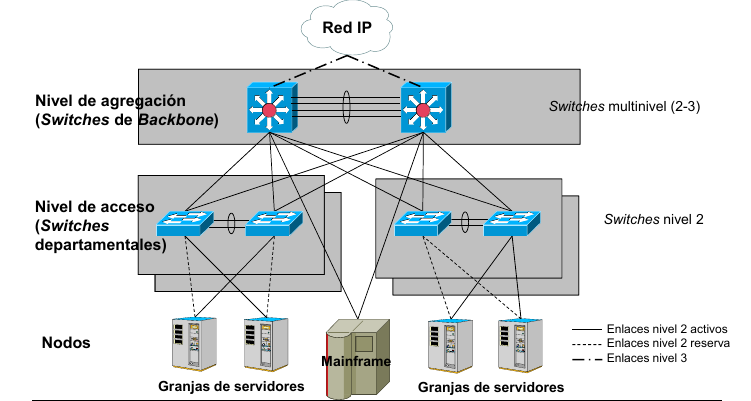
\includegraphics[width=\linewidth]{img/niveles.png}
\end{center}

La instalación de redundancias en el nivel 3 implica el uso de un protocolo de encadenamiento dinámico (OSPF, BGP), igual que en el caso de redes de área extendida (WAN).

A nivel 2, implica la aparición de bucles en los posibles caminos entre dos nodos de la red lo que lo hace incompatible con el protocolo \textit{Transparent Bridging} empleado en Ethernet. Este problema se resuelve con el \textit{Spanning Tree Protocol}, que se mejoró con el \textit{Rapid Spanning Tree Protocol}. Para optimizar el uso de VLANs se deben crear múltiples \textit{spanning trees}, solución proporcionada por \textit{Multiple Spanning Tree}.

En definitiva, si en la red de comunicación tenemos redundancias en un determinado nivel, es necesario emplear un protocolo que permita encontrar el mejor camino de un elemento a otro aún con las redundancias.

\subsection{Rapid Spanning Tree Protocol, RSTP}

Al aplicar este protocolo tenemos cada switch asociado a un identificador que nos da su prioridad. El de mayor prioridad (menor identificador, ID1) se denomina switch raíz. El siguiente en prioridad se le denomina switch raíz alternativo (ID2).

Para cada puerto hay que determinar de que tipo es:
\begin{itemize}
\item Raíz. Da el mejor camino al switch raíz

\item Designado. Proporciona a cada segmento de red conectado al switch el mejor camino al switch raíz. Es decir, que para algún nodo, su mejor camino hasta el nodo raíz implicar coger justo este enlace.

\item Alternativo. Otros.
\end{itemize}

Periódicamente, cada switch genera una \textit{Bridge Protocol Data Unit, BDPU} y la envía a todos los switches de la red.

\textcolor{red}{Mirar el ejemplo de moodle subido por la profesora. Explica bastante bien el protocolo}

\subsection{Detección de fallos en RSTP}
Puede producirse un fallo en un enlace conectado a un RP o DP, que se detecta directamente por los switches que forman el enlace; o puede darse un fallo en un switch. Si hay tres turnos seguidos en los que no se recibe BDPU de un switch, se le da por muerto.

Tras el fallo, todos los switches reconfiguran el spanning tree, mediante intercambios locales de los switches afectados por el cambio y el resultado se propaga al resto de la red.

\obs Hay otra versión de este mecanismo es el \textit{spanning tree normal}, en el que únicamente el root bridge transmite BPDU. Sólo se detecta un problema tras 20 segundos (vida máxima) y tras esto recalculamos el spanning tree completo.

\subsection{Redundancia en la conexión de servidores a nivel 2}
La redundancia básica en la conexión de un ordenador a una LAN se consigue mediante el uso de dos o más adaptadores de red.

Los puertos de estos adaptadores (un puerto por adaptador) tendrán la misma MAC, pero sólo uno de los adaptadores estará disponible. Si cae, el sistema activará otro. No afecta a los protocolos de niveles superiores.

\begin{defn}[EtherChannels]
Consiste en la agrupación de enlaces Ethernet donde todos los puertos poseen la misma MAC como si fuesen sólo 1 (y así lo ven desde arriba) y están activos simultáneamente.

Da mayor rapidez en la resolución de fallos y mejora el ancho de banda pero su implementación es costosa. Se requiere que ambos extremos de la conexión tengan soporte de \textbf{EtherChannels}. Los componentes de un \textbf{EtherChannel} no se pueden disgregar para conectar varios dispositivos distintos. A todos los efectos, es un único enlace.

\end{defn}

\subsection{Redundancia de las WAN}
Las redes WAN permiten establecer la interconexión entre elementos distantes de sistemas distribuídos. Se basan en el protocolo TCP/IP y se distinguen dos tipos de componenetes: enlaces y unidades de encadenamiento (routers).

La alta disponibilidad de las WAN se consigue teniendo muchos routers y enlaces para que siempre haya caminos alternativos. La gestión del tráfico a través de las diferentes rutas se lleva a cabo con los protocolos de encadenamiento dinámico que estudiamos en Redes: OSPB y BGP.

\begin{defn}[OSPF]
Protocolo de encadenamiento dinámico eficaz y ampliamente utilizado en redes IP. Se basa en el conocimiento de toda la red y el empleo de Dijkstra para localizar el camino más corto. Se organiza la red en áreas dentro de las cuales los routers encaminan los paquetes. Para cambiar de área se emplean los Area Border Gateways (routers fronterizos)

El mensaje OSPF Hello se emplea para conocer la topología de la red con lo que cada router conoce a sus vecinos. Y con el mensaje Link State se informa del estado de los enlaces.
\end{defn}

Se puede producir un fallo en OSPF por la caída de un enlace, que se deteca de forma inmediata, por la caída de un router, que se detecta gracias al protocolo OSPF Hello, que sirve de \textit{keep-alive}. El mensaje Hello se intercambia cada 10 segundos. Si tras cuatro rondas no se han recibido Hello's de un router, se le da por muerto.

Si en un caso concreto se requiere una configuración estática (estaciones de trabajo, por ejemplo) el router por defecto que se asigna a estos dispositivos se convierte en un SPOF (Single Point Of Failure). Para evitarlo se emplea un cluster de routers controlado con el protocolo \textit{Virtual Router Redundancy Protocolo, VRRP}

\begin{defn}[VRRP]
Protocolo de \textit{clustering} para routers empleado para proporcionar redundancia en routers en los casos en que representan un punto único de fallo en rutas de la red. El router se sustituye por un \textit{virtual router} formado por un router activo y otro en \textit{stand-by}.

El router de mayor prioridad será el activo y asume como propias una dirección IP y una MAC que habrán sido asignadas al router virtual. Si cae el router se activa otro.
\end{defn}

El router activo envía mensajes Hello en \textit{multicast} cada x segundos. Si transcurre un tiempo predefinido sin recibir mensajes Hello se da al router por muerto y se activa el siguiente en prioridad. Este tiempo de espera predefinido es menor cuanto menor sea la prioridad. Así cuando esté un router activo que no sea el inicial, tendrá más probabilidades de que se le de por muerto, por lo que el router principal tendrá más probabilidades de volver.

En el \textbf{fail-back} hay dos opciones:
\begin{itemize}
\item Si la configuración activa preempt, el router de mayor prioridad asume el tráfico. Supone una breve interrupción del servicio mientras se produce el cambio.
\item Si la configuración desactiva preempt, se deja el router actual como activo hasta un posible fallo, quedando el reincorporado como router de backup.
\end{itemize}

\begin{defn}[Balanceador de carga]
Un balanceador de carga es un dispositivo capaz de distribuir peticiones entre un grupo de servidores para su proceso. Tiene como objeto aumentar la capacidad de proceso y la disponibilidad del servicio.

Previamente se realizaba este proceso en redes IP a través del DNS, resolviendo el mismo nombre por distintas IP pero esto no garantizaba que el servidor estuviera activo y los cambios del DNS son lentos al propagarse por la red.

Frente a un switch que sólo maneja información de nivel 2 y un router que sólo maneja información a nivel 3, el \textbf{Load Balancer, LB} también utiliza información de los niveles de transporte y aplicación para realizar el encadenamiento. Como mínimo debe garantizar que en TCP todos los paquetes de la misma conexión van al mismo servidor.
\end{defn}

Para emplear un LB, se asigna una dirección IP virtual (VIP), puerto y protocolo para el servicio a prestar; se asocian al LB los servidores que prestan el servicio y se definen unos mecanismos de distribución de carga y entrega de paquetes.

Cuando llega una petición, el LB decide qué servidor debe atenderla y se la reenvía. El servidor procesará la petición y devolverá una respuesta que será reenviada al cliente. Este último paso, según la configuración de entrega de paquetes, puede eliminarse siendo el servidor quien directamente responde al cliente. (Direct Server Return vs Destination NAT)

El mecanismo de distribución de carga puede ser cualquiera: Round Robin, alterno, menor número de conexiones, ponderado, mejor tiempo de respuesta, por origen de la petición, etc.

En cualquier caso es necesario considerar condiciones límite para realizar la entrega:
\begin{itemize}
\item Máximo número de conexiones permitido
\item Umbral de tiempo de respuesta
\item \textbf{Gracefull Shutdown}. No mandar más mensajes a un servidor que quiere desconectarse
\item \textbf{Tiempo de gracia}. Tiempo que se deja a un servidor desde que está activo hasta que se le envía tráfico, para permitir su estabilización adecuada.
\end{itemize}

Si todos los paquetes de respuestas pasaban por el LB, se puede detectar un fallo si un servidor deja de responder, se puede monitorizar en \textit{handshake} de TCP o los códigos de retorno de HTTP. Si no es así, se emplean pruebas de nivel 3 con ICMP echo/replay; a nivel 4, con apertura/cierre de conexiones TCP; o pruebas de nivel 7, tratar de conectar con la aplicación. Estos acciones las realizaría el LB para comprobar que el servidor esté activo.

El LB debe ser capaz de hacer que un cliente se conecte siempre a un mismo servidor para que se mantenga la sesión, que no está implementada de modo estándar en TCP/IP. Existen diferentes formas de hacerlo:
\begin{itemize}
\item Aplicando un algoritmo de balanceo por origen. Tiene el problema de que si varios clientes están tras una NAT son indistinguibles en este sentido.
\item Por concurrencia de conexiones. Una nueva petición de un cliente se envía al mismo servidor que mantiene la actual
\item Cookies o identificadors SSL que guarden información de la sesión. Requiere analizar el paquete e impide que el balanceo se haga por paquete. Es necesario partir la conexión TCP en el LB
\end{itemize}

\subsection{Redundancia en los sistemas de almacenamiento de la información}
La información es el punto más crítico de todo sistema informático puesto que perder datos o no tenerlos disponibles adecuadamente puede ser fatal para cualquier tipo de negocio.

La redundancia de este tipo de elementos es más compleja pues es necesario mantener la consistencia y garantizar que los elementos de procesamiento redundantes accedan a la misma copia de la información.

Existen diferentes arquitecturas de almacenamiento. Veamos algunas:
\begin{itemize}
\item \textbf{Conexión direta (Direct Attached Storage, DAS)}. Consiste en conectar el dispositivo de almacenamiento directamente al servidor o estación de trabajo, es decir, físicamente conectado al dispositivo que hace uso de él. Normalmente se usa directamente el protocolo SCSI en alguna de sus variantes.

\item \textbf{Conexión a red (Network Attached Storage, NAS)}. Es el nombre dado a una tecnología de almacenamiento dedicada a compartir la capacidad de almacenamiento de un computador (Servidor) con computadoras personales o servidores clientes a través de una red (normalmente TCP/IP), haciendo uso de un Sistema Operativo optimizado para dar acceso con los protocolos CIFS, NFS, FTP o TFTP.

\item \textbf{Red de área de almacenamiento (Storage Area Network, SAN)}. Red dedicada al almacenamiento que está conectada a las redes de comunicación de una compañía. Además de contar con interfaces de red tradicionales, los equipos con acceso a la SAN tienen una interfaz de red específica que se conecta a la SAN. Utiliza fibra óptica como medio de transporte y el protocolo \textit{FibreChannel}

\item \textbf{Internet SCSI (iSCSI)} Estándar que permite el uso del protocolo SCSI sobre redes TCP/IP

\item \textbf{FibreChannel Over IP (FCIP)} Encapsula el protocolo FibreChannel sobre IP estableciendo túneles FC sobre TCP.

\item \textbf{Internet Fibre Channel Protocol (iFCP)} Implementa FC sobre IP pero no en modo túnel sino interpretando el protocolo FC.
\end{itemize}

Uno de los métodos para mantener redundante la información en unos ciertos discos es el uso de \textbf{Redundan Array of Independen Disks, RAID}, que ya hemos estudiado en otras asignaturas.

\begin{center}
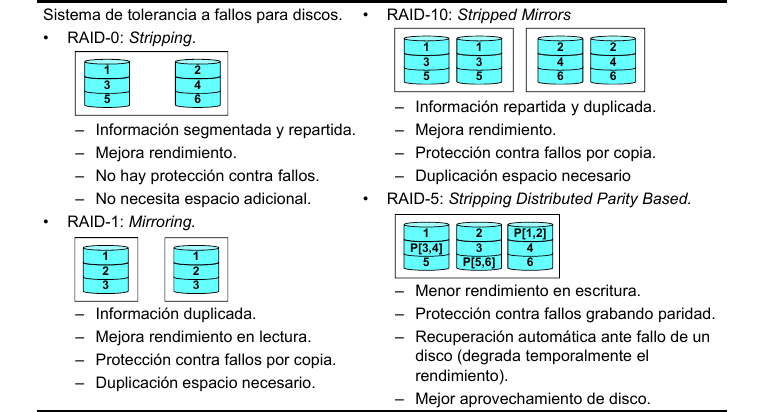
\includegraphics[width=\linewidth]{img/raid.png}
\end{center}

Los servidores de disco proporcionan herramientas autónomas para garantizar la copia de la información, y garantizar así su disponibilidad para los servidores que la utilizan, liberando así a los servidores de aplicaciones de la tarea de realización de las copias.

Estas copias pueden ser locales o remotas. Estas últimas podrían ser síncronas o asíncronas.

Dentro de las copias locales existen dos tipos: clonación de discos (se copia la información de una Unidad Lógica\footnote{Viene a ser como las particiones lógicas pero que afectan a diferentes discos, no sólo a 1} a otra) y las copias instantáneas (\textit{Snapshots o Flash Copy}).

\begin{defn}[Flash Copy]
Copia de una Unidad Lógica en el instante que se solicita, copiando los punteros a los sectores que contienen la información.

En caso de que haya una actualización de un sector, se copia la información antigua y se actuliza el puntero de la copia instantánea.

Se emplean para generar una copia consistente de la información en un momento preciso para su uso posterior.

\obs Básicamente guardas un puntero a la posición guardada. Si no la modifican, pues ya lo tienes. Si se modifica esa parte del disco, mueves la antigua información a otro sitio y actualizas tu puntero.
\end{defn}

Las copias remotas \textbf{síncronas} consisten en que la actualización de la información del servidor primario se copia a los secundarios y el proceso no finaliza hasta que no se ha actualizado la información en todos los servidores, lo que da lugar a una alta latencia de escritura. \textbf{Empleado para realizar copias locales que garanticen la alta disponibilidad}

En las \textbf{asíncronas}, una vez se actualiza el primario se guardan los cambios en un buffer y se van aplicando en el resto de servidores mediante un proceso en paralelo. Requiere un protocolo de sincronización. \textbf{Empleado para realizar copias remotas que permitan la recuperación ante desastres} \href{http://searchdatacenter.techtarget.com/es/consejo/Ventajas-e-inconvenientes-de-la-replicacion-remota-en-la-recuperacion-de-desastres}{Leer más}

Las posibles averías en discos físicos individuales son resueltas por la arquitectura RAID. Si se producen averías en una Unidad Lógica (LUN) completa o en un servidor de disco se siguen los siguientes pasos:
\begin{enumerate}
\item[1] \textbf{Fail-Over}. Se interrumpe la copia remota y la LUN secundaria pasa a principal. Para ello se notifica al servidor de proceso que debe usar a LUN secundaria y se comienza a registrar los cambios.

\item[2] \textbf{Fail-Back} Se copia el secundario activo al primario una vez recuperado. Para ello se detiene el trabajo del servidor de proceso, se reestablece la copia y se notifica al servidor de proceso que puede seguir utilizando el primario.
\end{enumerate}


\subsection{Redundancia en los sistemas de proceso}
Este tipo de redundancia se consigue mediante la asociación de los elementos de proceso (servidores) en grupos (clusters) que realizan una tarea común.

Cada servidor ejecutará un determinado número de grupos de servicio compuesto por una identidad de red (direcciones a las que el servicio responde), un conjunto de información almacenada en discos físicos o LUNs y un conjunto de procesos.

Si un servidor de un cluster falla, los grupos de servicio que soporta deben ser trasladados a otro elemento del cluster.

Básicamente un grupo de servicios es un conjunto de actividades que desempeña un servidor, es decir, procesos que ejecuta, direcciones a las que responde y memoria que usa. Si el servidor cae y no puede desempeñar estas actividades, otro tiene que ocupar su lugar.

Hay tres tipos de clusters según su modo de funcionamiento y gestión.
\begin{enumerate}
\item[1] \textbf{Clusters Activo-Pasivo o asimétricos:} Cada grupo de servicio se ejecuta en un nodo. Existen nodos de reserva en stand-by para ejecutarlos en caso de fallo.

\begin{defn}[Heartbeat]
In computer clusters, heartbeat network is a private network which is shared only by the cluster nodes, and is not accessible from outside the cluster. It is used by cluster nodes in order to monitor each node's status and communicate with each other.

Es uno de los puntos críticos de un \textit{cluster} de alta disponibilidad. Si falla se producirá la activación simultánea de ambos nodos, generando conflicos y caída del servicio.

Puede implementarse como una red de área local o mediante la escritura en una sección reservada de disco compartido.
\end{defn}

Para aumentar la fiablidiad del \textbf{heartbeat} se pueden tomar diversas medidas:
\begin{itemize}
\item Eliminar SPOF en los mecanismos de transporte del heartbeat.
\item Emplear dos heartbeat (dos redes o red+disco). Actuar sólo en caso de fallo
de ambos.
\item Emplear redes independientes lo más simples posibles: cable cruzado para
dos nodos, o segmentos de LAN con switches independientes.
\item Vigilar el correcto funcionamiento de los procesos que generan y atienden los
hearbeats en cada nodo. Instalar un watchdog local que los rearranque en caso de caída.
\end{itemize}

Existe una serie de \textbf{problemas a la hora de rearrancar en el servidor secundario} en el caso de fallo de uno de los nodos.

Si el cambio en la dirección IP se realiza sobre un adaptador con otra dirección MAC, la caché ARP de los clientes mantendrá la antigua hasta que detecten la nueva situación. Por ello se asume también la antigua dirección MAC.

Cuando la parada es no planificada (se dió un fallo en el sistema) se perderán datos de las aplicaciones, las cachés de disco y/o transacciones que se estuvieran realizando. Es por ello que el arranque de servicios en el servidor de reserva se hace siguiente los procedimientos de arranque tras un cierre anormal:
\begin{itemize}
\item Revisión de la consistencia de los sistemas de archivos a nivel de sistema operativo.
\item Revisión de la consistencia de los datos en disco a nivel de aplicación (por ejemplo, bases de datos).
\item Rollback de las transacciones activas en el momento del fallo.
\end{itemize}

En caso del fail-back este proceso será planificado, realizándose un cierre ordenado. En ambos casos se interrumpirá el servicio.

\item[2] \textbf{Clusters Activo-Pasivo cruzados o simétricos:} Cada grupo de servicio se ejecuta en un nodo. Todos los nodos ejecutan grupos de servicio. En caso de fallo de un nodo, el resto se hacen cargo de la ejecución de sus grupos de servicio.

El modelo es similar al anterior, pero con grupos de servicios activos en ambos nodos. Cada nodo tiene direcciones de servicio fijas y, en caso de fallo, el resto de nodos deberá hacerse cargo de todas las direcciones.

En este modelo nunca se parará el sistema y, si no hay fallo, hay menos capacidad de proceso desaprovechada.

Por otro lado, este modelo tiende a sobrecargar los nodos y, debido a la carga de trabajo de los supervivientes tras un fallo, es posible que les cueste absorber la carga del nodo caído. Además, es imposible asignar dos o más direcciones MAC en el adaptador de un nodo de modo que los clientes del nodo caído deberán realizar un nuevo ARP para conectar con otro nodo.


\item[3] \textbf{Clusters Activo-Activo:} Cada grupo de servicio se ejecuta en múltiples nodos. El fallo de uno de los nodos no supone la caída del grupo de servicio.

En este modelo existe un mecanismo de balanceo de carga para asignar las peticiones de los clientes a alguno de los nodos activos, que realiza el reparto de la carga y la verificación de la actividad.

Si falla uno nodo no cae el grupo de servicio e incluso, dependiendo del tipo de aplicación, las conexiones activas en el momento del fallo pueden mantenerse también.

El cluster debe incluir soluciones para el acceso compartido a discos en lectura y escritura, creación de áreas de memoria compartida entre los nodos del cluster, consistencia de la información distribuída entre los distintos nodos, etc.

\begin{example}
Ya vimos en el tema 2 la arquitectura de un servidor de aplicaciones J2EE, que es la que muestra la siguiente imagen:
\begin{center}
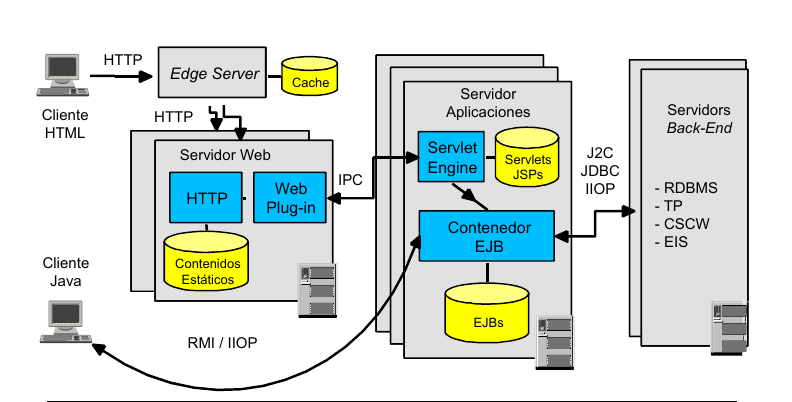
\includegraphics[width=\linewidth]{img/j2ee.png}
\end{center}

Se trata de un \textbf{cluster Activo-Activo}.

El balanceo de carga entre servidores Web lo realiza el Edge Server y el balanceo de carga entre Servlet Engines lo realiza el Web Plug In.

La alta disponibilidad en el acceso a los contenedores EJB y a los servicios de Back End es proporcionada por IIOP (corba) y por mecanismos de \textit{clustering} respectivamente.

La continuidad de la sesión entre distintas Servlet Engines se obtiene mediante el mantenimiento común de los datos de sesión. Este soporte común se puede conseguirse mediante una tabla de sesiones en una BD compartida, un gestor de réplica centralizado (Redundado para evitar SPOF) o un gestor de réplica distribuído.
\end{example}

\end{enumerate}

\section{Recuperación ante desastres}

Un desastre es cualquier circunstancia que puede producir un fallo en la operativa del negocio de una empresa. Pueden ser naturales, humanos, accidentes ...

Aunque tengan poca probabilidad, el impacto puede ser muy alto (por ejemplo, si se queman tus servidores de datos). Para garantizar la recuperación ante un desastre no basta con las técnicas de alta disponibilidad vistas hasta ahora sino que son necesarias nuevas técnicas que se presentan en esta sección.

Veamos algunas definiciones necesarias para entender los conceptos que analizaremos en este apartado:

\begin{defn}[Recovery\IS Point Objective (RPO)][Recovery\IS Point Objective]\index{RPO}
Instante de tiempo al que se es capaz de recuperar la información existente en el sistema tras un fallo. Si no es 0, habrá perdida de datos
\end{defn}

\begin{defn}[Recovery\IS Time Objective (RTO)][Recovery\IS Time Objective]\index{RTO}
Tiempo que se tarda en recuperar los sistemas tras producirse un fallo. Si no es 0, habrá interrupciones de servicio.
\end{defn}

Menores valores de RTO y RPO requieren mayor coste por lo que hay que analizar bien las necesidades del servicio.

Hay unas reglas básicas en el diseño de arquitecturas tolerantes a desastres:
\begin{enumerate}
\item Proteger datos y nodos de proceso mediante distribución geográfica.

Cuanto más alejados se encuentren, mayor seguridad, pero mayor
complejidad y coste.

\item Proporcionar a los CPDs redundancia en el suministro de energía.
Preferiblemente con acometidas independientes, a través de rutas alternativas de
distribución y proporcionadas por distintas entidades suministradoras.

\item Proporcionar a los CPDs redundancia en el acceso de telecomunicaciones. Con
las mismas consideraciones que en el caso anterior.

\item Generar copias consistentes de la información, garantizando la capacidad de
recuperar los datos desde ellas.
\begin{itemize}
\item \textbf{Copias off-line:} backups en cinta. Proporcionan un RPO elevado.

Puesto que hay que hacerlos de forma consistente, debe detenerse las aplicaciones mientras se realiza el backup o emplear técnicas de copia instantánea.

Además debe probarse que la información se restaura correctamente.

\item \textbf{Copias on-line:} réplicas directas de disco a disco. Proporcionan un RPO reducido.

Los mecanismos más habituales, ordenados de menor a mayor fiabilidad son:
\begin{enumerate}
\item Scripts de usuario. Automatizados por planificador.
\item Réplicas basadas en software en los sistemas de proceso, a distintos niveles:

\item Réplicas basadas en nivel de driver: mirroring remoto.
\item Réplicas basadas en el hardware de los servidores de disco: síncronas y
asíncronas, estudiadas previamente.
\end{enumerate}
\end{itemize}

\end{enumerate}

\subsection{Arquitecturas de CPDs orientadas a la recuperación ante desastres}
\textbf{Clusters a nivel de campus}
\begin{itemize}
\item Los elementos del cluster se distribuyen entre dos edificios próximos.
\item Extensión de LAN y SAN entre ambos edificios, normalmente con cableado propio.
\item Es posible la copia síncrona de información entre servidores de disco.
\item El funcionamiento lógico es como un cluster local: Proporciona alta disponibilidad.
\item Protege frente a desastres que ocurran en un único edificio.

\end{itemize}

\textbf{Clusters metropolitanos}
\begin{itemize}
\item Similar al anterior, pero con edificios en ubicaciones distantes que no excedan el rango en el que es posible realizar copia síncrona de la información.
\item Extensión de LAN y SAN con enlaces alquilados de alta velocidad (“fibra oscura”, WDM).
\item Protege frente a desastres locales.

\end{itemize}

\textbf{Clusters contienentales}
\begin{itemize}
\item Sin límite de distancia entre centros.
\item Requieren conexión a través de red WAN.
\item Protege frente a desastres en áreas extensas (región o estado), según la distancia entre centros.

\end{itemize}
\newpage
\textbf{Soluciones mixtas}
\begin{itemize}
\item Cluster local o metropolitano para garantizar alta disponibilidad, añadiendo un cluster continental para garantizar recuperación ante desastres.

\end{itemize}

\begin{center}
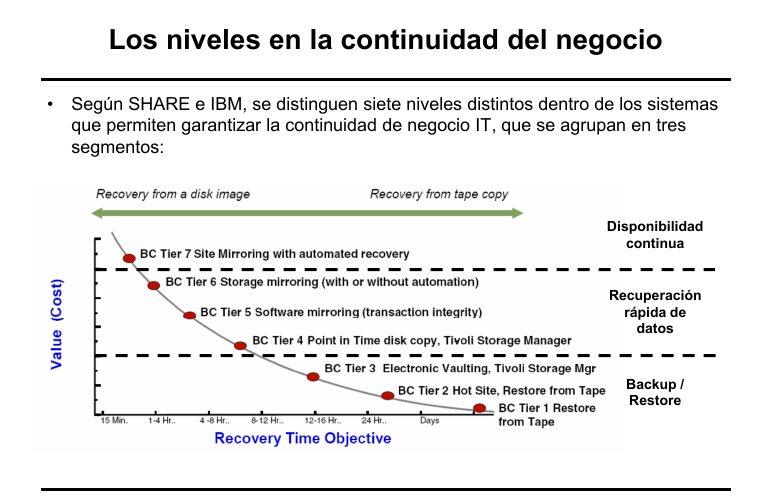
\includegraphics[width=\linewidth]{img/continuidad_negocio.png}
\end{center}

\newpage
\section{Problemas Tema 3}
\begin{problem}[1]
Se dispone de un equipo con un MTTF de 500 horas, que se encuentra bajo un contrato de mantenimiento que garantiza su reparación en un tiempo medio de 10 horas.
  \ppart El proveedor nos ofrece sustituirlo por un equipo de mayor calidad, con un MTTF de 1000 horas. Calcular la mejora de disponibilidad que supone este cambio.
  \ppart Tras un tiempo trabajando con el nuevo equipo, el proveedor nos ofrece de nuevo un nuevo equipo de mucha mayor calidad, con un MTTF de 2000 horas. Calcular la mejora de disponibilidad que supondría el nuevo cambio respecto al segundo equipo.

%%%%%%%%%%%%%%%%%%%%%%%%%%%%%%%%%%%%%%%%%%%%%%%%%%%%%%%%%%%%%%%%%%%%%
\solution
\textcolor{red}{Hecho por Edu}

\spart
  Calculemos la \textit{availability} de cada equipo:
  \[ A_1 = \frac{500}{500+10} = \frac{50}{51} \approx 0.98039 \]
  \[ A_2 = \frac{1000}{1000+10} = \frac{100}{101} \approx 0.990099 \]
  Luego la mejora es inferior al 1\%.

\spart
  \[ A_3 = \frac{2000}{2000+10} = \frac{200}{201} \approx 0.995 \]
  Lo que supone una mejora inferior al 0.5\% respecto al segundo y un 1.5\% respecto al original.

\end{problem}

%%%%%%%%%%%%%%%%%%%%%%%%%%%%%%%%%%%%%%%%%%%%%%%%%%%%%%%%%%%%%%%%%%%%%
\begin{problem}[2]
Se desea prestar un servicio con una indisponibilidad menor de 10 horas por
año.
  \ppart Calcular la disponibilidad deseada del sistema.
  \ppart Se dispone de un servicio de mantenimiento que es capaz de sustituir un equipo averiado en 24 h.\\
Calcular el MTTF que debe tener el equipo para poder satisfacer el requerimiento de disponibilidad establecido.

  \ppart Si sólo se dispone de equipos con un MTTF de 2000 horas, calcular el número de equipos que se deberían colocar en paralelo para garantizar el requisito.

%%%%%%%%%%%%%%%%%%%%%%%%%%%%%%%%%%%%%%%%%%%%%%%%%%%%%%%%%%%%%%%%%%%%%
\solution


\end{problem}

%%%%%%%%%%%%%%%%%%%%%%%%%%%%%%%%%%%%%%%%%%%%%%%%%%%%%%%%%%%%%%%%%%%%%
\begin{problem}[3]
El servidor de envío de mensajes ("busca") descrito en el problema número 7 del Tema 2 (\ref{tema2:prob7}) se compone de dos dispositivos: uno de recepción de mensajes y otro de difusión de los mismos.
\begin{itemize}
\item El MTTF del dispositivo de recepción de mensajes es de 1000 horas, y
\item el MTTF del dispositivo de difusión es de 1500 horas.
\end{itemize}
Ambos los atiende el mismo servicio técnico, que en ambos casos nos asegura un MTTR de 5 horas.\\

Calcular la disponibilidad total del sistema.

%%%%%%%%%%%%%%%%%%%%%%%%%%%%%%%%%%%%%%%%%%%%%%%%%%%%%%%%%%%%%%%%%%%%%
\solution



\end{problem}

%%%%%%%%%%%%%%%%%%%%%%%%%%%%%%%%%%%%%%%%%%%%%%%%%%%%%%%%%%%%%%%%%%%%%
\begin{problem}[4]
Los datos de disponibilidad de cada uno de los componentes de la red de la entidad financiera descrita en el problema número 8 del Tema 2 (\ref{tema2:prob8}) son los siguientes :
\begin{itemize}
	\item MTTF del multiplexor: 2000 h.
	\item MTTF del servidor: 2000 h.
	\item MTTF de cada terminal remoto: 1000 h.
	\item MTTF de la línea de comunicaciones del terminal remoto: 500 horas.
	\item MTTR de todos los elementos: 5 horas.
\end{itemize}

Suponiendo la existencia de dos únicos terminales remotos, realizar el diagrama de bloques de disponibilidad y calcular la disponibilidad global del sistema.

%%%%%%%%%%%%%%%%%%%%%%%%%%%%%%%%%%%%%%%%%%%%%%%%%%%%%%%%%%%%%%%%%%%%%
\solution



\end{problem}

%%%%%%%%%%%%%%%%%%%%%%%%%%%%%%%%%%%%%%%%%%%%%%%%%%%%%%%%%%%%%%%%%%%%%
\begin{problem}[5]
Un servidor de fecha y hora de una red se compone de dos elementos, que deben estar operativos para
atender el servicio: Un ordenador, que satisface las peticiones, y un receptor
de señales horarias externo, que permite obtener la hora exacta. Si ambos equipos
tienen un MTTF de 1500 horas, calcular el MTTR mínimo que debemos considerar,
supuesto igual en ambos, si se desea una disponibilidad total del servicio mayor del 99\%.

%%%%%%%%%%%%%%%%%%%%%%%%%%%%%%%%%%%%%%%%%%%%%%%%%%%%%%%%%%%%%%%%%%%%%
\solution



\end{problem}

%%%%%%%%%%%%%%%%%%%%%%%%%%%%%%%%%%%%%%%%%%%%%%%%%%%%%%%%%%%%%%%%%%%%%
\begin{problem}[6]
Un  servicio que debe tener una disponibilidad mínima de 0.99
se debe proporcionar con un sistema cuyo tiempo medio hasta el fallo es de
 2000 horas.
\begin{enumerate}
	\item Calcular el tiempo medio para reparar el equipo que es necesario para satisfacer la disponibilidad solicitada.
	\item Al comenzar con la explotación del servicio se descubre que el
programa que lo implementa tiene fallos que hacen que en ocasiones se
bloquee, dejando de atender peticiones. Para resolverlo es necesario
detener el proceso y volverlo a arrancar. Se ha estimado que en media se
 produce un fallo cada dos días. El fallo se tarda en descubrir un
promedio de 5 min. y la reiniciación del proceso requiere, también en
promedio, 7 min. Calcular la disponibilidad del sistema considerando este
 efecto.
	\item Suponiendo imposible modificar el programa o cambiar el equipo,
proponer una alternativa que permita, en las nuevas circunstancias,
satisfacer el requerimiento inicial de disponibilidad.
\end{enumerate}

%%%%%%%%%%%%%%%%%%%%%%%%%%%%%%%%%%%%%%%%%%%%%%%%%%%%%%%%%%%%%%%%%%%%%
\solution



\end{problem}

%%%%%%%%%%%%%%%%%%%%%%%%%%%%%%%%%%%%%%%%%%%%%%%%%%%%%%%%%%%%%%%%%%%%%
\begin{problem}[7]
Una petición que se procesa en un servidor web tiene que pasar por
cuatro clases de elementos distintos para su resolución completa. Estos
elementos son:
  \begin{itemize}
    	\item Un distribuidor de carga, que reparte las peticiones a los servidores web.
    	\item Un servidor web, que entrega al cliente páginas estáticas e
imágenes. Existen en el sistema tres servidores web, de igual
funcionalidad, pudiendo cualquiera de ellos atender las peticiones.
    	\item Un servidor de aplicaciones, que ejecuta programas bajo petición
 de los servidores web. El sistema posee dos de estos servidores, de
igual funcionalidad. Los servidores web pueden enviar indistintamente
sus peticiones a cualquiera de ellos.
    	\item Un servidor de base de datos, al cual acceden los programas que
se ejecutan en los servidores de aplicaciones para recuperar los datos
que necesitan para realizar las peticiones.
  \end{itemize}


  Es necesario, por tanto, que esté disponible al menos un elemento
de cada una de las clases citadas anteriormente para que el sistema
completo funcione.
  \begin{enumerate}
    	\item Dibujar el diagrama de disponibilidad del sistema total definido.
    	\item Suponiendo que todos los ordenadores que implementan los
servidores tienen la misma disponibilidad, A, y que cada servidor se
implementa en un ordenador distinto, calcular la expresión de la
disponibilidad total del sistema, AT en función de A.
    	\item Calcular el valor numérico de AT cuando el tiempo medio entre
fallos es de 2000 horas y el tiempo medio entre reparaciones, 100 horas.
  \end{enumerate}

%%%%%%%%%%%%%%%%%%%%%%%%%%%%%%%%%%%%%%%%%%%%%%%%%%%%%%%%%%%%%%%%%%%%%
\solution



\end{problem}

%%%%%%%%%%%%%%%%%%%%%%%%%%%%%%%%%%%%%%%%%%%%%%%%%%%%%%%%%%%%%%%%%%%%%
\begin{problem}[8]
Cada uno de los elementos que componen el servidor de transacciones descrito en el problema número 15 del Tema 2 (\ref{tema2:prob15}) se ejecuta en un ordenador independiente que tiene un MTTF de 4000
horas. Calcular el MTTR necesario para garantizar una disponibilidad del sistema total del 99.9\%.

%%%%%%%%%%%%%%%%%%%%%%%%%%%%%%%%%%%%%%%%%%%%%%%%%%%%%%%%%%%%%%%%%%%%%
\solution



\end{problem}

%%%%%%%%%%%%%%%%%%%%%%%%%%%%%%%%%%%%%%%%%%%%%%%%%%%%%%%%%%%%%%%%%%%%%
\begin{problem}[9]
Comparar desde el punto de vista de disponibilidad las dos soluciones propuestas en el problema número 18 del Tema 2 (\ref{tema2:prob18})
 para resolver un cuello de botella en acceso a disco. Suponer que todos
 los discos empleados tienen los mismos MTTF y MTTR, y justifique qué
alternativa es más fiable calculando y comparando las disponibilidades
en ambos casos.

%%%%%%%%%%%%%%%%%%%%%%%%%%%%%%%%%%%%%%%%%%%%%%%%%%%%%%%%%%%%%%%%%%%%%
\solution


\end{problem}

%%%%%%%%%%%%%%%%%%%%%%%%%%%%%%%%%%%%%%%%%%%%%%%%%%%%%%%%%%%%%%%%%%%%%
\begin{problem}[10]
Los servidores de directorios DSA1 y DSA2 descritos en el problema número 20 del Tema 2 (\ref{tema2:prob20})
 se encuentran conectados por una línea de comunicaciones que tiene una
disponibilidad de 0.99. La disponibilidad de DSA2 es de 0.98. Si el MTTF
 de DSA1 es de 2000 horas, ¿cuál será el MTTR que deberemos garantizar
para él, para conseguir que la disponibilidad del sistema total sea
igual a 0.95? ¿Cuál sería, en este caso, la disponibilidad de DSA1
considerado aislado del resto del sistema?

%%%%%%%%%%%%%%%%%%%%%%%%%%%%%%%%%%%%%%%%%%%%%%%%%%%%%%%%%%%%%%%%%%%%%
\solution


\end{problem}

%%%%%%%%%%%%%%%%%%%%%%%%%%%%%%%%%%%%%%%%%%%%%%%%%%%%%%%%%%%%%%%%%%%%%
\begin{problem}[11]
Se desea definir la arquitectura de un servidor de aplicaciones
 siguiendo el modelo estándar visto en la asignatura, compuesto por
cuatro elementos distintos en la cadena de procesamiento:
\begin{itemize}
	\item Capa de distribución: Balanceador de carga del tráfico de usuarios.
La alta disponibilidad de estos elementos se garantizará mediante el
protocolo VRRP.
	\item Capa de presentación: Servidores web. La capa anterior garantiza una alta disponibilidad activo-activo en esta capa.
	\item Capa de aplicación: Servidores de aplicaciones. El web plug-in
insertado en los servidores web garantiza la alta disponibilidad
activo-activo en esta capa.
	\item Capa de datos: Servidores de bases de datos. Se elige que la
alta disponibilidad de esta capa la proporcione un cluster
activo-pasivo.

\end{itemize}

Los ordenadores con los que se trabaja tienen un MTTF de 4000 horas, y su MTTR es de 48 horas.
\begin{enumerate}
	\item Calcular la disponibilidad de la capa de presentación si se colocan en ella dos servidores web.
	\item Adicionalmente a los posibles problemas de hardware reflejados
en el MTTF genérico de los servidores empleados, se han detectado fallos
 en el software de los servidores de aplicaciones, que hacen que en
promedio exista un fallo por semana que hace necesario rearrancar el
servidor. El tiempo de rearranque del servidor es de 30 min. Calcular la
disponibilidad de la capa de aplicación si se colocan en ella dos
servidores de aplicaciones.
	\item En el caso de la base de datos, la recuperación tras un fallo
no se realiza a través de las reparaciones habituales, sino que se
dispone de un cluster activo-pasivo. El tiempo de conmutación al
servidor pasivo se compone de los siguientes tiempos:
\begin{itemize}
	\item Tiempo de detección del fallo en el servidor principal: 30s.
	\item Tiempo de arranque del servidor pasivo: 30 mn.
	\item Tiempo de recuperación de la base de datos tras un cierre anormal, en el caso peor: 2 horas.

\end{itemize}

Calcular la disponibilidad de la capa de datos en dicho caso peor.
	\item En la capa de distribución se conocen los siguientes datos:
\begin{itemize}
	\item Advertisement interval (tiempo entre la transmisión de paquetes hello por el balanceador activo): 1s.
	\item Master down interval (tiempo tras el cual si no se reciben paquetes hello se considera el master caído): 3s.
	\item Skew adicional para producir la conmutación tras la expiración del master down interval: 0.

\end{itemize}

Calcular, en el caso peor, la disponibilidad del conjunto de dos balanceadores de carga trabajando en esta configuración.
	\item Calcular la disponibilidad total de la instalación.
\end{enumerate}

%%%%%%%%%%%%%%%%%%%%%%%%%%%%%%%%%%%%%%%%%%%%%%%%%%%%%%%%%%%%%%%%%%%%%
\solution


\end{problem}

\printindex
\end{document}

